\documentclass{book}

\usepackage{url}
\usepackage{cite}
\usepackage{anysize}
\usepackage{graphicx}
\usepackage{listings}
\usepackage{exercise,chngcntr}
\usepackage{listings}
\usepackage{color}
\usepackage{graphicx}
%http://en.wikibooks.org/wiki/LaTeX/List_Structures#Inline_lists
\usepackage{paralist}

% The following commands make LaTeX not consider the periods in a few
% abbreviations as periods at the end of sentences.
\newcommand*{\eg}{e.g.\@}
%
\newcommand*{\ie}{i.e.\@}
%
\makeatletter
%
\newcommand*{\etal}{\@ifnextchar{.}{et al}{et al.\@}}
%
\makeatother

% The following commands should be used to define key and value pairs.
\newcommand{\Def}[2]{\expandafter\newcommand\csname rmk-#1\endcsname{#2}}
%
\newcommand{\Use}[1]{\csname rmk-#1\endcsname}

% Wraps notes on what needs to get fixed.
\newcommand{\Fix}[1]{\textcolor{red}{[#1]}}

% Wraps junk text.
\newcommand{\Comment}[1]{}

% Wraps good text that needs to be excluded, e.g., due to space limits.
\newcommand{\Space}[1]{}

\newcommand{\FigRef}[1]{Figure~\ref{#1}}

\newcommand{\SecRef}[1]{Section~\ref{#1}}

\newcommand{\Code}[1]{\texttt{#1}}

\graphicspath{{26Snipes_Images/}}
\DeclareGraphicsExtensions{.pdf, .png, .ps, .PNG}   % NOT .jpg  because it throws away the detail.

\definecolor{dkgreen}{rgb}{0,0.6,0}
\definecolor{gray}{rgb}{0.5,0.5,0.5}
\definecolor{mauve}{rgb}{0.58,0,0.82}

\lstset{frame=tb,
  language=Java,
  aboveskip=3mm,
  belowskip=3mm,
  showstringspaces=false,
  columns=flexible,
  basicstyle={\small\ttfamily},
  numbers=none,
  numberstyle=\tiny\color{gray},
  keywordstyle=\color{blue},
  commentstyle=\color{dkgreen},
  stringstyle=\color{mauve},
  breaklines=true,
  breakatwhitespace=true,
  tabsize=3
}

\counterwithin{Exercise}{chapter}
\counterwithin{Answer}{chapter}

\marginsize{1in}{1in}{1in}{1in}

\newcommand\CodingSpectator{\textsc{CodingSpectator}}

\newcommand\Fluorite{\textsc{Fluorite}}

\newcommand\CodingTracker{\textsc{CodingTracker}}

\newcommand\Performed{\texttt{performed}}

\newcommand\Canceled{\texttt{canceled}}

\newcommand\Unavailable{\texttt{unavailable}}

\Def{NumberOfEclipseAutomatedRefactorings}{33}

\Def{NumberOfCodingSpectatorSupportedRefactorings}{23}



\usepackage{url}
\usepackage{cite}
\usepackage{anysize}
\usepackage{exercise,chngcntr}
\usepackage{listings}
\usepackage{color}
\usepackage{graphicx}

\graphicspath{{images/}}
\DeclareGraphicsExtensions{.pdf, .png, .ps}   % NOT .jpg  because it throws away the detail.

\definecolor{dkgreen}{rgb}{0,0.6,0}
\definecolor{gray}{rgb}{0.5,0.5,0.5}
\definecolor{mauve}{rgb}{0.58,0,0.82}

\lstset{frame=tb,
  language=Java,
  aboveskip=3mm,
  belowskip=3mm,
  showstringspaces=false,
  columns=flexible,
  basicstyle={\small\ttfamily},
  numbers=none,
  numberstyle=\tiny\color{gray},
  keywordstyle=\color{blue},
  commentstyle=\color{dkgreen},
  stringstyle=\color{mauve},
  breaklines=true,
  breakatwhitespace=true
  tabsize=3
}

\counterwithin{Exercise}{chapter}
\counterwithin{Answer}{chapter}

\marginsize{1in}{1in}{1in}{1in}


\begin{document}

\title{ASD}

\chapter{A Practical Guide to Analyzing IDE Usage Data\vspace{-0ex}}
\author{
Will Snipes, Emerson Murphy-Hill,
Thomas Fritz, \\
Kostadin Damevski,
Anil R. Nair, David Shepherd
}
\maketitle
\thispagestyle{empty}
\pagestyle{empty}

\section{Abstract}
As software development evolved, Integrated Development Environments (IDEs) sprang up to aid the developer in managing the ever increasing complexity of software programs.  Meant to increase productivity, modern IDEs such as Eclipse and Visual Studio provide tools and capabilities to perform tasks such as navigating among classes and methods, continuous compilation, code refactoring, automated testing, and integrated debugging.  The breadth of development activities supported by the IDE makes collecting editor, command, and tool usage data valuable for analyzing developers’' work patterns.  

Prior work in the RSSE book on Collecting and processing data for recommendation systems provides a description of tools, analysis methods, and important findings from developer usage data analysis.  The RSSE chapter is also a great introduction to prior research applying usage data to solve issues that challenge developers.  In this chapter, we will provide a practical how-to description for collecting and analyzing usage data from IDEs.  Each topic will provide practical guidance with how-to examples and exercises.  We also provide a role-based view of analysis describing what a software engineering researcher can do with the data, what a developer can do, and what toolsmiths can learn from the data.

Instrumenting the IDE to collect usage data and observing developers’' work through ethnographic studies gives researchers a greater level of detail on developers’' work than previously possible. Instrumenting the IDE involves extending the IDE within the provided API framework.  Eclipse and Visual Studio support a rich API framework allowing logging of many commands and actions  as they occur.  Tools used for research that instrument the Visual Studio IDE include Hackystat\cite{V:johnson2003beyond}, Blaze, and Codealike.  Tools that instrument the Eclipse IDE include Mylyn Monitor, CodingSpectator, Hackystat\cite{V:johnson2003beyond}, and Zorro\cite{Kou2010Operational}.

Assembling IDE usage data across developers and temporally across many development sessions allows researchers to study differences and similarities in work patterns.   Raw usage data must be transformed to answer specific research questions.  Techniques to transform usage data include classification, attribute extraction, deriving sequences, state-based models, and  multi-event sequences.  

Usage data supports analysis of how developers spend their time\cite{V:johnson2003beyond}, what activities might benefit from greater tool support \cite{V:MurphyHill2012How}, where developers have difficulty comprehending code \cite{Carter2010Are}, even whether they are following specific practices such as test-driven development\cite{Kou2010Operational}.  Combining usage data with additional data dimensions such as change history or code analysis, researchers can understand larger influences of low-level developer practices.  With these data we can answer questions such as the level of expertise developers have for an area of source code. \cite{Fritz2010Degreeofknowledge}

Currently, few developers study their own work habits with such data.  However, in a world of devices such as fitbit \footnote{fitbit device to track physical activity www.fitbit.com}, we may see self-analysis play a more important role.  By studying their own usage patterns, developers may learn how to improve their own practices or help their peers advance.

There are limits, however, to what IDE usage data can tell us.  The missing elements include things like how well the developer knows the subject code base, what their mental model of the code is, or how they intend to alter the code to suit new requirements.  The developers'' experience, design ideas, and constraints they keep in mind during an implementation activity are factors that we must obtain separately.  

Looking forward, usage data from development environments provides a platform for greater understanding of developer's low-level practices.  We expect to uncover more nuggets of how developers create mental models, how they investigate code, how they perform mini trial and error experiments, and what might release further productivity improvements for everyone.


\section{What Is Usage Data and Why Analyze It?}

types of data
	-tool usage
	-resource usage (file/method/etc)
	-click streams

need for analysis
	-answers questions about how developers work
	-example questions
	-who
		-researchers
		-toolsmiths
		-users (?)

benefits
	-understanding that you don't get from lab experiments. more realistic data
	-you can also use it in the lab, but screencast is also inefficent in storage and analysis
\section{How to Collect Data}



\subsection{ Data sources}
    \begin{itemize}
    \item
	- usage data from tools of course
\item
	- usage data in user study smaller setting is augmented by user explicit feedback to establish ground truth (e.g. search result was good) 
\item
	- smaller studies can ask questions about user activities that add rationale to the usage data that tells why user is doing what they are doing
\item 
	- small studies can generate a metric you can use with larger data source that does not have augmented data.  E.g. structured navigation that Robillard did supports a larger study such as what we did at ABB.
    \end{itemize}

\subsection{ Building Data Collection} 
  \label{BuildingDataCollection}

	Tailoring usage data collection to specific needs helps optimize the volume of data and privacy concerns when collecting information from software development applications.  While a general solutions described in the next sections collect all events from the Integrated Development Environment (IDE), limiting the data collection to specific areas for research can improve the result.  A process for defining the desired data can follow structures such as Goal-Question-Metric \cite{basili-GQM}  that refines a high-level goal into specific metrics to generate from data.  For example, to study the navigation practices of developers, we perfrom the GQM process as follows:
    \begin{itemize}
\item 
	Goal
\subitem 
	To assess and compare the use of structured navigation by developers in our study
\item 
	Possible Question(s)
\subitem
	What is the frequency  of navigation commands developers use when modifying source code?
\subitem
	What portion of navigation commands developers use are structured navigation rather than unstructured navigation?
\item
	Metric
\subitem
	Navigation Ratio is the proportion of the number of structured navigation commands used to the number of unstructured navigation commands used by a developer in a given time period (e.g. a day)

	    \end{itemize}

The next step is selecting the data to collect from the IDE related to the Metric defined for Navigation Ratio.  For this we identify the  commands related to structured navigation (in Visual Studio) as follows:
\begin{itemize}
\item 
 Navigate To (Ctrl+,) is a fuzzy search interface that lists identifiers matching the selected string 
\item Go To Definition (F12) brings up the code that defines the selected identifier 
\item View Call Hierarchy (Ctrl+K Ctrl+T) provides a two way analysis of an identifier's dependencies and uses
\item Class View (Ctrl+W, C) provides a browser and search function for classes and class hierarchy
\item Find All References (Ctrl+K,R) provides a list of lines that reference an identifier
\item Navigate to Event Handler in the XAML editor shows the event handler for an object
\item View Class Diagram generates a class diagram 
\item View Object Browser is a search tool and browser
\end{itemize}

Next we identify the commands related to unstrctured navigation as follows:
\begin{itemize}
\item selecting a file in an explorer window
\item selecting the tab for a file
\item using arrow and page up/down keys to go up/down through a file
\item scrolling, 
\item clicking on a file element
\item using GoTo Line command
\item using Find In Files command
\item using Quick Find command
\end{itemize}

These identified commands form the set of actions that usage data needs to collect to calculate the navigation ratio metric.  Notice that the commands are a mixture of defined actions within the tool and actions that result from mouse actions such as selecting a window or a window tab.  The latter need further refinement to determine how the usage monitor can identify these actions from available events in the IDE.  This is discussed in further detail in section \ref{buildItYourself}.

Assessing commands within a time duration (e.g. day) requires that we collect a time-stamp for each command.  Simply using the time as a "by variable" where we stratify data according to time is a straight-forward conversion.  The time-stamp can be converted to a date allowing data to be grouped by the day of the events.  Similarly the time-stamp can be convered to hour to look at events each hour of any given day.
Calculating duration or elapsed time for a command or set of commands adds new requirements to monitoring.  Specifically, the need to collect events that relate to when the application or IDE is being used and when it is not and the need to collect additional events that occur when the user has moved on from the command of interest.  This is discussed in further detail in section \ref{buildItYourself}.

Concerns over privacy intrusion makes usage monitoring a flash point for some people.  Privacy concerns can be divided into concerns about what data is collected that may expose the user or parts of the source code to prying eyes and who the data and aggregates of it are shared with.  

To alleviate concerns about what data is collected, steps such as hashing sensitive pieces of information can reduce the concern. If you collect information like window titles they can contain filenames, web site titles, or even email titles.  Hashing these names provides a measure of assurance that the data are less easily identifiable with the user of the system and with sensitive subjects they may be working on.   Collecting a user identification makes this data very helpful for understanding distribution of practices, however, this makes it more sensitive as well.  Generating an anonymous identifier to identify distinct users helps alleviate the concern that data will be associated with the user.

To reduce concerns about who the data are shared with, create a statement of policy around this.  If the data is for research purposes only, you can state specifically whom will have access to the data and what they will do with it.  Limiting statements such as not reporting data at the individual level helps this policy reduce concerns about who the data is shared with.


    \begin{itemize}
\item
      What data is relevant to collect? (data granularity depends on needs of subsequent analysis and anticipated space and time overhead; collecting aggregate data vs. individual events; mention that data should be timestamped as a lot of subsequent analyses depend on that)
    \item
      How to modify existing tools to collect data? (events are a good communication paradigm; centralizing the logger in the code allows for consistent log messages and easy maintenance; trade-offs in storing logs as highly structured or somewhat unstructured data)
    \item
      Privacy and anonymity considerations when collecting data. (what not to collect, using hashes to protect user identities)
      
     
    \item
    	Existing usage data (Mylyn's 99 developers, UDC, etc). %Emerson 
     
    \end{itemize}

\subsection{Instrumenting the IDE -- Using an Existing Framework} %Emerson
  
\begin{enumerate}
	\item 
	There are many existing frameworks to use. We suggest picking on and building off one. (Note: Clone these on github? include packaged with IDE?)
	
	\item Eclipse: Mylyn Monitor. Format: What it was originally intended to be used for. What data it collects. Where to get it. How to install it (w/version info). Example output. Deployment(?)
	
	\item CodingSpectator %https://github.com/vazexqi/CodingSpectator	
	
	\item Hackystat\cite{V:johnson2003beyond}, %https://code.google.com/p/hackystat/

	\item Zorro\cite{Kou2010Operational}. %same as Hackystat? How about VS tool?
	
	\item CodeAlike has one, too, but they get the data!
	
	\item Romain Robbes -- maybe for Visual Studio, but for smalltalk? SHould be in chapter.
\end{enumerate}

This section shows how to implement a usage data collection tool for Visual Studio that generates the Navigation Ratio metric (See \ref{BuildingDataCollection}) daily, giving the developer insight into his own navigation patterns. Readers attempting the tutorial should be familiar with C\# and .NET commands as well as have a working knowledge of Visual Studio.  

The lifecycle and threading behavior of this extension is straightforward for the sake of this tutorial. It starts when Visual Studio starts and continuously collects events as the user works, saving all data to a local file.  This example extension does not perform any background processing, thus the user may notice a delay during Visual Studio startup.  

This extension utilizes the Visual Studio Automation Object Model API, which is available to Visual Studio Extensions. Using this model we can access the Command object, which allows us to observe user commands that occur in Visual Studio by registering an event handler for each command. Thus, we can log commands relevant to the Navigation Ratio. 

Many extensions require configuration, as does this extension. The first time this extension runs, it creates a configuration file specifiying which events to record and how to classify those events (e.g., as structured or unstructured navigation).  The extension will create a new time-stamped log file each time it starts and record the events for that execution of Visual Studio in the log file. 

\subsubsection{Creating a Visual Studio Extension}

\begin{enumerate}
\item {\bf Install the Visual Studio SDK} - To create Visual Studio Extensions specialized libraries (e.g., the automation library) are needed, and thus the Visual Studio SDK must be installed.

\item {\bf Create a Visual Studio Solution and Project} - Using the 'New Project' wizard create a new project and solution in C\# by selecting Extensibility and Visual Studio Packageas shown in Figure \ref{fig:ProjectCreation}.  
\begin{figure}
	\centering
	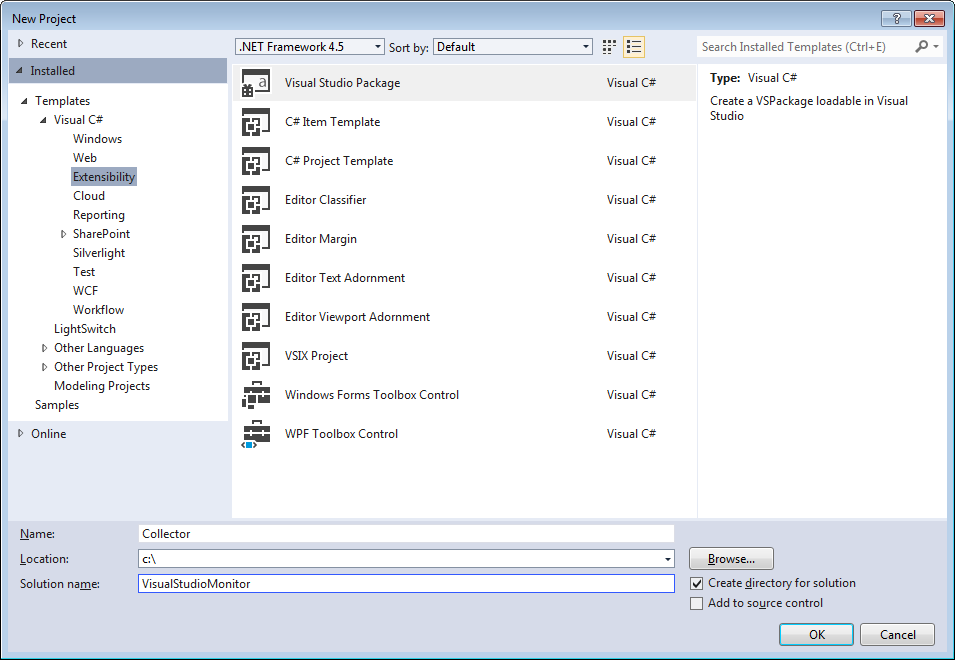
\includegraphics[width=4in]{CreateVSIXExtension.png}
	\caption{Create a Visual Studio Extension}
	\label{fig:ProjectCreation}
\end{figure}

Use "Collector" as the project name and "VisualStudioMonitor" as the solution name, then follow the default options for the first 2 steps of the wizard.  In the third step, when asked to specify what type of extension, select the option to generate a menu command.  Next, give the menu command a name of "Stop Monitoring" and a command ID of "StopMonitoring".  This menu option will allow the user to halt collection of data if they wish without quitting Visual Studio.  Click next on the next step and then Finish to setup your extension solution project.


After creating the project and solution, the solution explorer should look like figure \ref{fig:SolutionExplorer} showing the project files necessary for the extension to work.
\begin{figure}
	\centering
	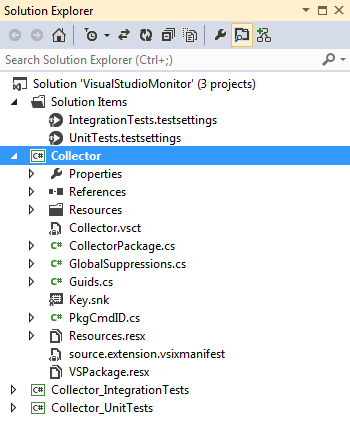
\includegraphics[width=2.5in]{SolutionExplorer.png}
	\caption{Solution Explorer with Visual Studio Extension}
	\label{fig:SolutionExplorer}
\end{figure}


\item {\bf Ensure the extension loads on startup} - The next step is to instruct the extension package to load when Visual Studio starts, by setting the attribute ProvideAutoLoad on the package class (CollectorPackage.cs). The GUID value in the below listing will load the package when Visual Studio starts.

\begin{lstlisting}
    // This attribute starts the package when Visual Studio starts 
    [ProvideAutoLoad("{ADFC4E64-0397-11D1-9F4E-00A0C911004F}")]
    [Guid(GuidList.guidCollectorPkgString)]
    public sealed class CollectorPackage : Package
\end{lstlisting}

\end{enumerate}

\subsubsection{Create Monitor Project}

In order to separate the Visual Studio Extension setup from the core functionality of the extension a second project should be created. We call this second project, part of the same solution, the Monitor project.

\begin{enumerate}
\item {\bf Create the Monitor project} - Add a class library type project to  the "VisualStudioMonitor" solution. Because the class library must be signed, go to the Properties for the Monitor project and select Signing from the list at the right.  In the Signing tab, check the "sign the assembly" checkbox then under "Choose a strong name key file", select Browse and browse over to the Key.snk file in the collector project (the file was created with the solution).

\item {\bf Create the monitoring class} - 
The next step is to create a static class that will manage the log file including starting, stopping recording data, and inserting data into the log file.  Rename the class created by Visual Studio in the Monitor project to "DataRecorder".    Because we don't want more than one recorder running at a time and want to access this class without instantiating it, make the class static.  Create a method to Start the recorder that generates a file name for the log file and sets a flag that the recording has started. A Stop method resets that flag and perhaps clears the file name.  A method to write a log message to the file completes DataRecorder.

\item {\bf Connecting the extension framework with the recorder} -
Finally, insert a call to DataRecorder.Start() at the end of the Initialize() method in the CollectorPackage class.  This will start the monitoring each time Visual Studio starts.  You will need to add a reference for the "Monitor" project to the Collector project, make sure you sign the Monitor project, then rebuild the solution.


The call to DataRecorder.Start() is inserted in the CollectorPackage as shown in Listing \ref{code:StartCall}.
\begin{lstlisting}[caption=Call to DataRecorder.Start(),label=code:StartCall]
        /////////////////////////////////////////////////////////////////////////////
        // Overridden Package Implementation
        #region Package Members

        /// <summary>
        /// Initialization of the package; this method is called right after the package is sited, so this is the place
        /// where you can put all the initialization code that rely on services provided by VisualStudio.
        /// </summary>
        protected override void Initialize()
        {
            Debug.WriteLine (string.Format(CultureInfo.CurrentCulture, "Entering Initialize() of: {0}", this.ToString()));
            base.Initialize();

            // Add our command handlers for menu (commands must exist in the .vsct file)
            OleMenuCommandService mcs = GetService(typeof(IMenuCommandService)) as OleMenuCommandService;
            if ( null != mcs )
            {
                // Create the command for the menu item.
                CommandID menuCommandID = new CommandID(GuidList.guidCollectorCmdSet, (int)PkgCmdIDList.StopCollector);
                MenuCommand menuItem = new MenuCommand(MenuItemCallback, menuCommandID );
                mcs.AddCommand( menuItem );
            }
            DataRecorder.Start();
        }
        #endregion
\end{lstlisting}

The source code for the DataRecorder.cs file is shown in Listing \ref{code:DataRecorder}
\begin{lstlisting}[caption=Data Recorder Class,  label=code:DataRecorder]
using System;
using System.Collections.Generic;
using System.Linq;
using System.Text;
using System.Threading.Tasks;

namespace Monitor
{
    public static class DataRecorder
    {
        public static void Start() {
            logDirectoryPath = System.IO.Path.GetTempPath();
            logFileName = System.IO.Path.Combine(logDirectoryPath, "collector " + DateTime.Now.ToString("yyyy-MM-dd HH.mm.ss") + ".log");
            try {
                using (System.IO.StreamWriter streamWriter = new System.IO.StreamWriter(
                    new System.IO.FileStream(logFileName, System.IO.FileMode.OpenOrCreate, System.IO.FileAccess.Write, System.IO.FileShare.ReadWrite)
                    ))
                {
                    streamWriter.WriteLine("Collector Started");
                }
            } 
            catch (System.IO.IOException ioexception) {
                Console.WriteLine("Error creating log file "+ioexception);
            }
         }

        public static void Stop() {

                WriteLog("Collector Stopped");
            
        
        }

        public static void WriteLog(string logToWrite)
        {
            try
            {
                using (System.IO.StreamWriter streamWriter = new System.IO.StreamWriter(
                    new System.IO.FileStream(logFileName, System.IO.FileMode.Append, System.IO.FileAccess.Write, System.IO.FileShare.ReadWrite)
                    ))
                {
                    streamWriter.WriteLine(logToWrite);
                }
            }
            catch (System.IO.IOException ioexception)
            {
                Console.WriteLine("Error writing to log file " + ioexception);
            }
        
        }

        private static string logFileName;
        private static string logDirectoryPath;
    }
}

\end{lstlisting}
\end{enumerate}

\subsubsection{Create the Data Model}

The next step creates a data model for storing and managing event monitoring for Visual Studio.  Because there are several different types of events, it makes sense to build an abstract class to manage the core data and use the Simple Factory pattern to generate each type of event monitoring.  With this pattern an abstract base class, called AbstractMonitoredEvent, provides common definitions for class fields that will be used for monitoring different Visual Studio events, conversion of those fields to and from the storage format, and (eventually) calling the WriteLog method in the recorder when the event fires.  This concrete class implements methods specific to Visual Studio commands that manages the fields available from the DTE.Command class.  The client in the Simple Factory pattern is a class that maintains the collection of events that either gets read from the file or queried from Visual Studio.   In this step we focus on the elements needed to store event information, and manage the configuration file data in XML format.

\begin{enumerate}
\item {\bf Implement the base class} - 
Create the AbstractMonitoredEvent class in the Monitor project in Visual Studio.  Then add data elements for EventName and Classification as follows.

\begin{lstlisting}
    [XmlInclude(typeof(MonitoredCommandEvent))]
    [XmlRoot(ElementName = "MonitoredEvent", Namespace = "http://Monitor")]
    public abstract class AbstractMonitoredEvent
    {
        /// <summary>
        /// Default constructor to use in serialization
        /// </summary>
        protected AbstractMonitoredEvent()
        {
        }

        public String EventName { get; set; }
        public String Classification { get; set; }
   }
\end{lstlisting}

So that we can store events in a configuration file then manipulate that configuration file later, we provision this abstract class for XML serialization of itself and its derived classes.  Dot NET attributes support the XML serialization in this structure.  The first attribute tells XML serialization that the MonitoredCommandEvent class is a derived class of AbstractMonitoredEvent that we will create next.  This provides the abiltiy to serialize and deserialize the public objects of the derived class by referencing the type of AbstractMonitoredEvent when creating a serializer.  The second attribute creates an XML namespace that all derived classes will share with the AbstractMonitoredEvent class.

\item {\bf Create the concrete subclass} - 
The next step is to create a derived class called MonitoredCommandEvent that inherits from AbstractMonitoredEvent.  MonitoredCommandEvent implements a constructor that builds a MonitoredCommandEvent object from the Command class of the DTE and a constructor that builds from an XElement.  An output method ToXElement translates the object to XML for saving.

After you create the class, add using statements for System.Xml.Serilization, and EnvDTE and their corresponding references in the project References configuration. 

The EnvDTE.Command object contains fields for Guid (a GUID string), ID and integer sub-id, and Name a readable name for the command.  To register an event handler for a EnvDTE.Command, you need get an object reference for the command using the Guid and ID to identify the command.  The GUID is  a Globally Unique IDentifier for command events in Visual Studio, however, some command events share a GUID and distinguish themselves with different EventIDs. Thus both elements are necessary to link a Command event from the DTE to an event hander in this extension.  The Name is useful information to understand what the command is.    There are several versions of the DTE object corresponding to versions of Visual Studio.  Depending on the commands of interest, each version may need to be queried for its commands.  

 The constructor that takes a Command as input, simply extracts the necessary and relevant fields from the DTE's Command object and transferrs the matching information into the corresponding fields from this class and the AbstractMonitoredEvent class.  


\begin{lstlisting}
    [XmlRoot(ElementName = "MonitoredEvent", Namespace = "http://Monitor")]
    public class MonitoredCommandEvent : AbstractMonitoredEvent {

         public int EventID { get; set; }
        public String Guid { get; set; }

        public MonitoredCommandEvent()
        {
        }

        public MonitoredCommandEvent(Command DTECommandObj) {
            if (DTECommandObj != null) {
                this.EventName = DTECommandObj.Name;
                this.Classification = EventName.Split('.')[0];  //use the first part of event name
                this.Guid = DTECommandObj.Guid;
                this.EventID = DTECommandObj.ID;
            }
            else {
                throw new ArgumentNullException("DTECommandObj");
            }
        }
\end{lstlisting}

 The attribute for XMLRoot is the same attribute assigned to the AbstractMonitoredEvent class which tells XML Serialization that this type is a type beloging to the abstract class.  In this class, create two public fields, EventID as int and GUID as string, that will save important information from the Visual Studio DTE object needed to engage monitoring for each command.  

\item {\bf Create the event factory}
To complete the Simple Factory pattern, a static factory class provides static factory methods that creates an object of type  MonitoredCommandEvent from a DTE Command object and returns it as an AbstractMonitoredEvent.  For now the only class to consider is the MonitoredCommandEvent derived class, however, a future step will add more derived classes.  
\end{enumerate}

\subsubsection{Query Save and Retrieve Visual Studio Command Event Info}

#insert intro about this section

\begin{enumerate}
\item {\bf Create the collection manager class} -
In this step, build the MonitoredEventCollection class that manages a List object of AbstractMonitoredEvent type.  The List object gets populated from an XML file that stores the configuration data.  The MonitoredEventCollection class provides a method to query the DTE for all commands and initialize the list.  Another method called after the DTE query stores the List contents in the same XML format file.  These two methods should be called in sequence the first time the extension launches. After that, it  reads the XML file on startup to initialize the List.  Call the method(s) to query, store and load the event list from the Start() method of the DataRecorder class in the previous step so that the Monitor will load the commands on startup.

Fortunately the DTE object has a query method that lists all the commands it manages.   The DTE Commands object returns an IEnumerable collection of EnvDTE.Command objects. The listing below provides a method to try to get an instance of the DTE.  It depends on references to EnvDTE, Microsoft.VisualStudio.Shell.12.0, and Microsoft.VisualStudio.OLE.Interop so be sure to add those to the project's References list.

%\begin{lstlisting}[caption=Method to get a DTE Reference,label=code:tryGetDTEObject,float=ht]
\begin{lstlisting}

		using EnvDTE;
		using Microsoft.VisualStudio.Shell; //12.0
		private static DTE tryGetDTEObject()
		{
			DTE dteobj=null;
			try
			{
				dteobj = ((EnvDTE.DTE)ServiceProvider.GlobalProvider.GetService(typeof(EnvDTE.DTE).GUID)).DTE;

			}
			//Important to catch the following exception if the DTE object is unavailable
			catch (System.Runtime.InteropServices.InvalidComObjectException)
			{} 
			//Important to catch the following exception if the DTE object is busy
			catch (System.Runtime.InteropServices.COMException)
			{}
			return dteobj;
		}

\end{lstlisting}

Once you have a reference to the DTE object from the tryGetDTEObject method, use the DTE to query the Commands  object.  Then process each command into the List managed by MonitoredEventCollection.  Example code to do this is shown below making use of the MonitoredEventFactory to generate each AbstractMonitoredEvent stored in the List.  The try-catch here is necessary because the saved DTE object could get disposed while the loop proceses the Commands.

\begin{lstlisting}
                try
                {
                    foreach (Command DTE_CommandEventObj in dteobj.Commands)
                    {
                        AbstractMonitoredEvent NewEvent = MonitoredEventFactory.GetMonitoredEvent(DTE_CommandEventObj);
                        if (NewEvent != null)
                        {
                            EventList.Add(NewEvent);
                        }
                    }
                }
                //This exception happens during dispose/finalize when VS exits, just return null
                catch (System.Runtime.InteropServices.InvalidComObjectException)
                {
                    return null;
                }
\end{lstlisting}

\item {\bf Enable persistence of the configuration} -
A persistent configuration file helps independently manage the events that get monitored for a study, and makes the configuration of all possible events easier to manage.    Using the framework's ToXelement methods, build methods in MonitoredEventCollection to save the List of AbstractMonitoredEvents to the configuration file and load them from the configuration file.  Below is the core code for the save to XML method that creates a serializer for the List object then writes that to the file stream.  Code for reading the XML file is left to the reader.

\begin{lstlisting}
                var serializer = new System.Xml.Serialization.XmlSerializer(typeof(List<AbstractMonitoredEvent>));
                using (Stream file = new FileStream(filepath, FileMode.Create, FileAccess.Write))
                {
                    serializer.Serialize(file, eventList);
                    file.Flush();
                }
\end{lstlisting}

\end{enumerate}


\newpage



\subsubsection{Register Event Handlers}

Now that the framework is complete and a configuration file for all command events to be monitored is ready, the methods to hook Visual Studio into event handlers that log each command can be created.  This step will add methods and member objects to AbstractMonitoredEvent and MonitoredCommandEvent classes to register event handlers with the DTE and dispose of them appropriately when necessary.  The MonitoredEventCollection class gets a new method to perform the registration from the objects in the list and another method to deregister them.

\begin{enumerate}
\item {\bf Define the registration interface } - 
The AbstractMonitoredEvent class should get a virtual RegisterEventForMonitoring method that takes an object parameter we will use to pass a DTE reference in.  The method returns a bool based on successful regisration.  The class also gets a non virtual Dispose() method  and a virtual Dispose(bool disposing) method with the former calling the latter and the latter setting a field isDisposed to true. This is the typical dispose structure.  Finally, the abstract class holds the non-virtual method to write the event log information (the abstract class's fields and a timestamp) to the log via the DataRecorder class.  This unifys logs for all derived classes into a common format.

\item {\bf Register individual commands} - 
The MonitoredCommandEvent class overrides the virtual RegisterEventForMonitoring method to implement registering an event handler for Command events.  Registering first must find the event in the DTE and assign it to the field, then attach a new event hander to the event.  Looking at the method listing below, the Guid and EventID are used as parameters to query the DTE Events object for the specific command event in this instance.  The result is assigned to a field, eventTypeObject.  Wiith this reference to the event, the next block adds an event handler that runs after the command is executed.  After all that if the eventTypeObject is not null, the method returns true for success.
\begin{lstlisting}
        public override bool RegisterEventForMonitoring(object dte)
        {
            if (!isDisposed && eventTypeObject == null && dte != null)
            {
                eventTypeObject = (dte as DTE).Events.get_CommandEvents(Guid, EventID) as CommandEvents;
            }
            if (eventTypeObject != null)
            {
                eventTypeObject.AfterExecute += new 
			_dispCommandEvents_AfterExecuteEventHandler(OnAfterExecute);
            }
            return (eventTypeObject != null);
        }
\end{lstlisting}

With the above method in Visual Studio, the missing fields and methods can be auto-generated via the "Generate" context menu command.  

The last step with MonitoredCommandEvent is to create the Dispose method that will deregister the event handler. This looks like the following:

\begin{lstlisting}
        protected override void Dispose(bool disposing)
        {
            if (eventTypeObject != null) 
		eventTypeObject.AfterExecute -= OnAfterExecute;
            this.isDisposed = true;
        }
\end{lstlisting}

Use the Visual Studio "Generate" command to generate a method stub for OnAfterExecute and the
code will compile.  In the OnAfterExecute method, call ToLog so the event data is captured in the log.

\item {\bf Register all commands} -  
MonitoredEventCollection now needs methods to perform registration and deregistration on all the events in the list.  As the following listing shows, RegisterEventInventoryForEventMonitoring() must get the DTE object then walk through the IDEEventListenerRegistry list calling the abstract method RegisterEventForMonitoring with the DTE.  If one of them succeeds then this method considers it successful.

\begin{lstlisting}
        public bool RegisterEventInventoryForEventMonitoring()
        {
            DTE dteobj = tryGetDTEObject();
            bool somethingRegistered = false;
            if (dteobj != null && IDEEventListenerRegistry != null && IDEEventListenerRegistry.Count > 0)
            {
                foreach (AbstractMonitoredEvent command in IDEEventListenerRegistry)
                {
                    if (command.RegisterEventForMonitoring(dteobj))
                    {
                        somethingRegistered = true;
                    }
                }
            }
            return somethingRegistered;
        }
\end{lstlisting}

The method in MonitoredEventCollection to de-register events in the List via Dispose() is left as an exercise for the reader to complete.

\item {\bf Connect to the package lifecycle} - 
Refactor the MonitoredEventCollection object in DataRecorder to a static class field.  Then add a call to RegisterEventInventoryForEventMonitoring() in the Start() method of DataRecorder.  Add a call to the de-register method of MonitoredEventCollection in the Stop() method of DataRecorder.  

\item {\bf Execute the extension} - 
Run the solution and use a few commands in Visual Studio, then give the Stop Collector command and check the log file.  You should see output like the following:
\begin{verbatim}
Collector Started
2014-02-02 13:46:52Z,Tools.AddinManager,Tools
2014-02-02 13:46:56Z,Tools.ExtensionsandUpdates,Tools
Collector Stopped
\end{verbatim}


\end{enumerate}


Below are descriptions of the code listings for the example code we discussed in this section.  Code listings are located at the end of the chapter.
\begin{itemize}
\item
The Listings for AbstractMonitoredEvent.cs in Code Listing \ref{code:AbstractMonitoredEvent_4}  show the additions to that class.  
\item
The listing for CommandMonitoredEvent.cs in Code Listing \ref{code:MonitoredCommandEvent_4} shows methods implemented for registration and disposal.
\item
The listing for MonitoredEventCollection.cs in Code Listing \ref{code:MonitoredEventCollection_4} shows list processing in calls to respective registration and de-registration methods for the List object.
\item
The DataRecorder class is shown in listing \ref{code:DataRecorder_4}.
\end{itemize}



\subsection{Classification of Events}
Now that the data collector is working, let's look at the classification of commands in Visual Studio according to the goal of understanding structured vs. unstructured navigation commands.  If you look at the generated XML file from MonitoredEventCollection, there are literally four thousand commands to choose from.  The sample program generates a base classification from the command family (usually a menu association), however, that does not distingush between navigation types.    The navigation events of interest relate to the prior stated metric Navigation Ratio.  For this metric,  we identify the  commands related to structured navigation (in Visual Studio) as follows:
\begin{itemize}
\item
 Navigate To (Ctrl+,) is a fuzzy search interface that lists identifiers matching the selected string
\item Go To Definition (F12) brings up the code that defines the selected identifier
\item View Call Hierarchy (Ctrl+K Ctrl+T) provides a two way analysis of an identifier's dependencies and uses
\item Class View (Ctrl+W, C) provides a browser and search function for classes and class hierarchy
\item Find All References (Ctrl+K,R) provides a list of lines that reference an identifier
\item Navigate to Event Handler in the XAML editor shows the event handler for an object
\item View Class Diagram generates a class diagram
\item View Object Browser is a search tool and browser
\end{itemize}

Next we identify the commands related to unstrctured navigation as follows:
\begin{itemize}
\item selecting a file in an explorer window
\item selecting the tab for a file
\item using arrow and page up/down keys to go up/down through a file
\item scrolling,
\item clicking on a file element
\item using GoTo Line command
\item using Find In Files command
\item using Quick Find command
\end{itemize}

These identified commands form the set of actions that usage data needs to collect to calculate the navigation ratio metric.  Notice that the commands are a mixture of defined actions within the tool and actions that result from mouse actions such as selecting a window or a window tab.  Now in the classification file generated from the tool, there is a field to classify each event.  Locating the events in the xml related to these commands and changing their classification to StructuredNav or UnstructuredNav will allow analaysis of the log data with respect to these classifications.

With this demonstration you see how to build a usage monitor for Visual Studio that records most commands the user can issue in the IDE.  What's missing?  Well there are other areas of the DTE to explore such as editor events, unit test events, build and debug session events that provide greater context to the user experience.  For brevity, capturing those events is left to the reader to explore on their own.

%\subsubsection{Unstructured Navigation Events}
%For this step, an important set of code is added to Monitor so users unstructured navigation actions can be captured.  Since unsturcutured navigation includes actions like scrolling through a soruce file or opening a source file from a project browser, the event collection requires a different part of the Visual Studio DTE api.  

%Add a reference to EnvDTE80 to get access to this portion of the API.  

%Add a reference to Microsoft.VisualStudio.TextManager.Interop to get access to the text editor manager.




\subsection{Eclipse Usage Data Collector}

This section outlines how to collect IDE usage data using Eclipse's Usage Data 
Collector (UDC).\footnote{\url{http://www.eclipse.org/epp/usagedata/}}
The UDC framework was originally build by the Eclipse Foundation, as a way to measure how the 
community was using the Eclipse IDE.
While UDC was included in official Eclipse releases and data was collected from
hundreds of thousands of Eclipse users between 2008 and 2011, the project was eventually shut down, 
and UDC was removed from official Eclipse releases.
However, the source code for UDC remains available and researchers can still use and deploy it.

\subsubsection{What Data is Collected}

The Eclipse Data Collector records the following types of Eclipse information:

\begin{itemize}
 
\item The runtime environment, such as the operating system and Java Virtual Machine.

\item Environment data, such as which bundles are loaded and when Eclipse
starts up and shuts down

\item Actions and commands that are executed, via menus, buttons, toolbars, and hotkeys.

\item Views, editors, and perspectives that are invoked.

\end{itemize}

\noindent
Let's look at an example of an event that UDC produces on a developer's machine:
\vspace{4mm}

\noindent
\begin{small}
\begin{tabular}{llllll}
\textbf{what}&\textbf{kind}&\textbf{bundleId}&\textbf{bundleVersion}&\textbf{description}&\textbf{time}\\
\hline
executed&command&org.eclipse.ui&3.7.0.v20110928-1505&org.eclipse.ui.edit.paste&1389111843130\\
\end{tabular}
\end{small}

\vspace{4mm}
\noindent
The first column tells us what kind of thing happened -- in this case, something was executed.
The second column tells us what was executed -- in this case, a command.
The third column tells us what bundle this event belonged to -- in this case, Eclipse's user interface bundle.
The fourth column gives us the version of the bundle.
The fifth tells us the name of the command that was executed -- in this case, paste.
The final column tells us when the command was executed, in Greenwich Mean Time -- in this case, January 7th, 2014 at 16:24:03 GMT.


\subsubsection{Limitations}

Apart from general limitations of collecting usage data (Section~\ref{sec:limitations}),
one significant limitation of UDC that we have found is that sometimes it has 
unexpectedly incomplete data.
For example, in planning for a study involving when people ran their JUnit tests,
we found that UDC recorded an event when the ``Run \textgreater~Run As \textgreater~Run as JUnit Test'' menu item was selected,
but not when the ``Run As'' button was pressed on the toolbar.
We suspect that the reason has to do with how different user interface accordances
invoke the same functionality.
In general, when you are planning on running a study with UDC, be sure to know what 
types of events you are looking for, and test them to make sure UDC captures those events.

\subsubsection{How to Use It}

Collecting data for your own research is fairly straightforward with Eclipse UDC,
and we describe how to do so here.
We also include an accompanying screencast that shows the 
basics.\footnote{\url{https://docs.google.com/file/d/0B7DV-T4_2mpKRWgwRnJnTWpvN0E/edit}}
%TODO move this screencast to youtube, once you're happy

\paragraph{Gathering Data Using the UDC Client.}

Let's talk about how data is collected on a developer's machine.
Since UDC was last included in the Eclipse Indigo SR2 
release,\footnote{(\url{http://www.eclipse.org/downloads/packages/release/indigo/sr2}}
if you have the option of which Eclipse to use, we recommend downloading
that version.
By default, UDC starts collecting data when Eclipse is start up. 
You can verify this by going to ``Windows \textgreater~Preferences'', then
select the ``Usage Data Collector'' item (Figure~\ref{fig:prefPage1}).
The \textit{Enable capture} option should be checked.

\begin{figure}
  \centering
  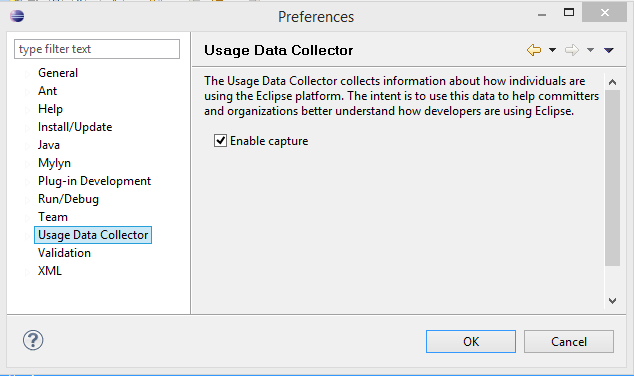
\includegraphics[scale=.58]{prefPage1}
  \caption{Eclipse Usage Data Collector preference page.}\label{fig:prefPage1}
\end{figure}

Before looking at the data, execute a few commands and open a few views 
in Eclipse.
Then, on your file system, open the following path as a subdirectory
of your current workspace (Figure~\ref{fig:filesystem}): 

\vspace{4mm}
\texttt{.metadata/.plugins/org.eclipse.epp.usagedata.recording}
\vspace{4mm}

\noindent
In that folder, depending on how many UDC events have been gathered,
a number of comma separated value (CSV) files will appear, where \texttt{upload0.csv} is the oldest
and \texttt{usagedata.csv} is the newest.
Open up \texttt{usagedata.csv} -- you should notice a large number and a variety of events.
Be sure to look specifically for events that you executed and views that you opened earlier.

\begin{figure}
  \centering
  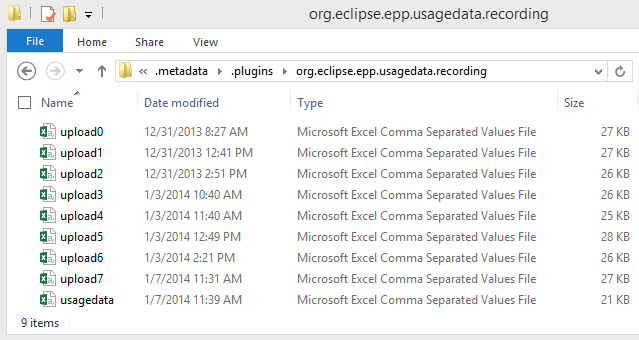
\includegraphics[scale=.58]{filesystem}
  \caption{UDC data files.}\label{fig:filesystem}
\end{figure}

Before doing a study, be aware that Eclipse will ask and periodically attempt to upload
data to the Eclipse foundation server.
You should \emph{not} allow it to do this, because each time data is uploaded, the underlying
CSV files are deleted.
Furthermore, because the UDC project is no longer officially supported, the official Eclipse
UDC server no longer accepts the data, so your usage data is, in effect, lost permanently.
Unfortunately, there is no easy way to tell the UDC client to permanently store
usage data.
An easy workaround is to increase the upload period to 90 days (Figure~\ref{fig:upload}),
which should be enough time to complete the experiment.
The long-term fix for this issue is to modify the source code, as we will explain
how to do shortly, to never upload data.

\begin{figure}
  \centering
  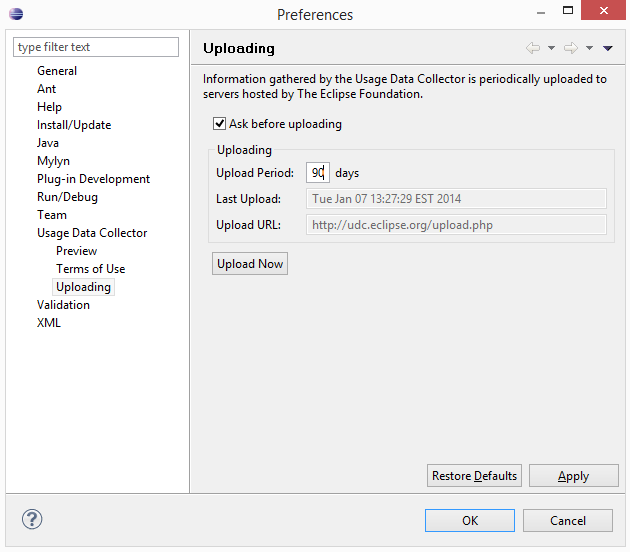
\includegraphics[scale=.58]{upload}
  \caption{Changing the UDC upload frequency.}\label{fig:upload}
\end{figure}

If you're doing a lab experiment, collecting data should be simply a matter of 
copying and deleting the CSV files after each participant has done the experiment.
You can append the files together or put them in a database for analysis.

\paragraph{Modifying the UDC Client.}

You may wish to modify the UDC client yourself, perhaps to add a custom filter for events
or to disable data uploading.
Whatever the reason, making modifications to the client is fairly easy.

The first step is to check out the UDC source code into your Eclipse
workspace using git.\footnote{\url{http://git-scm.com/}}
Here we will again use Eclipse Indigo SR2, but we will specifically be using the 
``Eclipse for RCP and RAP Developers'' download package because we will
modify Eclipse plugins.
Before importing the necessary plugins, we recommend switching to 
the Indigo SR2 tag, to assure compatibility with
Eclipse.
To do so, clone the git repository\footnote{\url{http://git.eclipse.org/c/epp/org.eclipse.epp.usagedata.git/}} 
locally, open up ``Tags'', right click on ``Indigo SR 2'',
then choose ``Checkout''.

To import the projects into Eclipse, right click on the repository, then click 
``Import Projects,'' then ``Import Existing Projects.''
The three core projects to import are:

\begin{itemize}
\item org.eclipse.epp.usagedata.internal.gathering
\item org.eclipse.epp.usagedata.internal.recording
\item org.eclipse.epp.usagedata.internal.ui
\end{itemize}

Next, we recommend a quick smoke test to determine whether you 
can actually make changes to the UDC client.
Open \texttt{UsageDataRecordingSettings.java}, then modify the value of \texttt{UPLOAD\_URL\_DEFAULT}
to \texttt{"my\_changed\_server"}.
Then, create a new debug configuration that is an Eclipse Application, and press 
``Debug'' (Figure~\ref{fig:debugconfig}).
Finally, you can verify that your change worked by going to UDC's Uploading 
preference page, noticing that the Upload URL is now ``my\_changed\_server''.

\begin{figure}
  \centering
  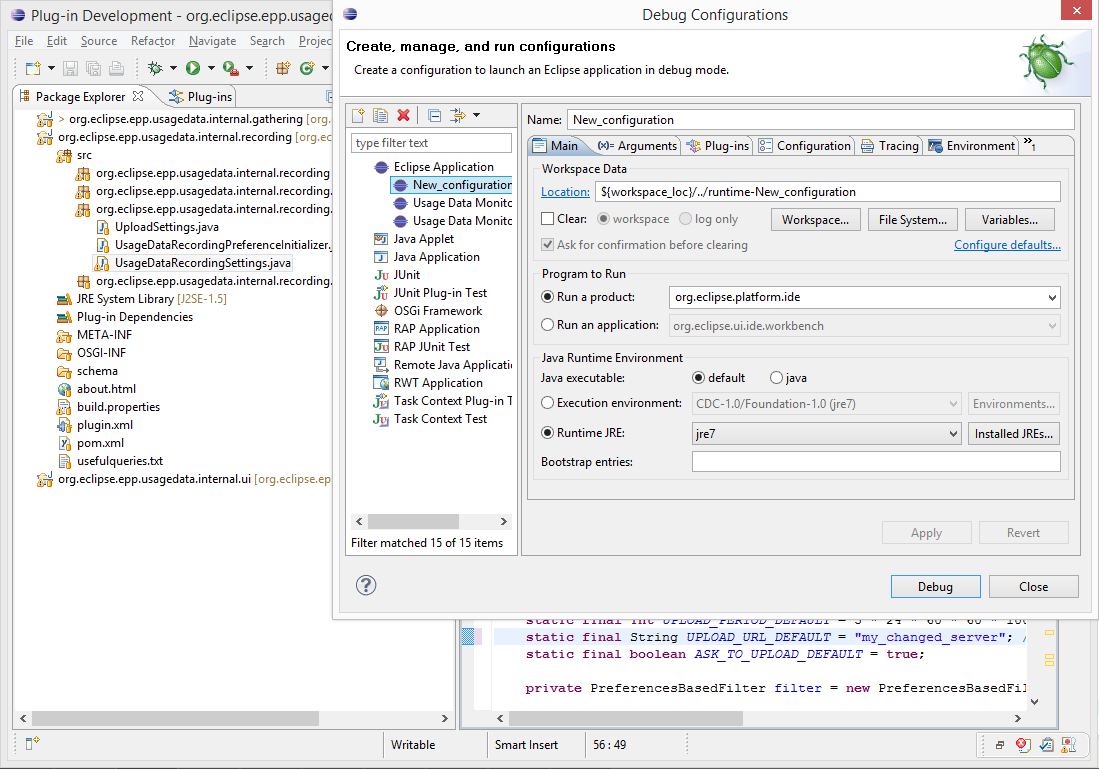
\includegraphics[scale=.58]{debugconfig}
  \caption{Debugging the UDC client.}\label{fig:debugconfig}
\end{figure}

From here, you can make any changes to the UDC client that you wish.
One thing you may want to do is upgrade UDC to work with more recent versions
of Eclipse.
The code is likely currently out of date
because it has not been maintained since the UDC project was shut down.
Another thing you may wish to do is deploy your new version of UDC via
an Eclipse update site to the developers you want to study.
There are many resources on the web for plugin deployment instructions,
such as Lars Vogel's tutorial on creating 
plugins.\footnote{\url{http://www.vogella.com/tutorials/EclipsePlugIn/article.html#deployplugin_tutorial}}

\paragraph{Transmitting Data over the Internet.}

If you do not plan on doing a lab study where you can manually collect UDC usage
files, you will want to have the UDC client send the data to you directly.
As we mentioned, the best way to do this is probably by changing the default
server URL in the client source code.
An easy way to change the server when debugging is by adding the following Java
virtual machine arguments:

\vspace{4mm}
\texttt{-Dorg.eclipse.epp.usagedata.recording.upload-url=http://localhost:8080}
\vspace{4mm}

\noindent
However, simply changing the client to point at a new URL is insufficient, 
because there actually has to be a working server at that URL, ready to 
receive UDC data.
While the source code of official Eclipse server was not officially made 
available, Wayne Beaton from the Eclipse Foundation unofficially released
some of the PHP code from the Eclipse Foundation's server.
If you would like to download that code, you will find it in our git repository.
%TODO need to put this code into git
However, our PHP skills are very basic and we were not immediately able
to get the server working as expected, but we expect that anyone familiar with
debugging PHP should be able to.

\newpage

Creating your own server that receives UDC data is fairly straightforward.
Let's create a simple one using Apache's HttpComponents library,
the same library that UDC uses to upload data.
Specifically, we can create a server by simply extending Apache's tutorial
web server.\footnote{\url{http://hc.apache.org/httpcomponents-core-ga/httpcore/examples/org/apache/http/examples/ElementalHttpServer.java}}
First, we'll need a generic request handler to wait for HTTP connections:

\begin{lstlisting}
import java.io.IOException;
import org.apache.http.ConnectionClosedException;
import org.apache.http.HttpException;
import org.apache.http.HttpServerConnection;
import org.apache.http.protocol.BasicHttpContext;
import org.apache.http.protocol.HttpContext;
import org.apache.http.protocol.HttpService;

/**
 * Based on
 * http://hc.apache.org/httpcomponents-core-ga/httpcore/examples/org/apache
 * /http/examples/ElementalHttpServer.java
 */
class WorkerThread extends Thread {

	private final HttpService httpservice;
	private final HttpServerConnection conn;

	public WorkerThread(final HttpService httpservice, final HttpServerConnection conn) {
		super();
		this.httpservice = httpservice;
		this.conn = conn;
	}

	@Override
	public void run() {
		System.out.println("New connection thread");
		HttpContext context = new BasicHttpContext(null);
		try {
			while (!Thread.interrupted() && this.conn.isOpen()) {
				this.httpservice.handleRequest(this.conn, context);
			}
		} catch (ConnectionClosedException ex) {
			System.err.println("Client closed connection");
		} catch (IOException ex) {
			System.err.println("I/O error: " + ex.getMessage());
		} catch (HttpException ex) {
			System.err.println("Unrecoverable HTTP protocol violation: " + ex.getMessage());
		} finally {
			try {
				this.conn.shutdown();
			} catch (IOException ignore) {
			}
		}
	}
}
\end{lstlisting}

\newpage
\noindent
We'll also need a generic request listener:

\begin{lstlisting}
import java.io.IOException;
import java.io.InterruptedIOException;
import java.net.ServerSocket;
import java.net.Socket;

import org.apache.http.HttpConnectionFactory;
import org.apache.http.HttpServerConnection;
import org.apache.http.impl.DefaultBHttpServerConnection;
import org.apache.http.impl.DefaultBHttpServerConnectionFactory;
import org.apache.http.protocol.HttpService;

/**
 * Based on
 * http://hc.apache.org/httpcomponents-core-ga/httpcore/examples/org/apache
 * /http/examples/ElementalHttpServer.java
 */
class RequestListenerThread extends Thread {

	private final HttpConnectionFactory<DefaultBHttpServerConnection> connFactory;
	private final ServerSocket serversocket;
	private final HttpService httpService;

	public RequestListenerThread(final int port, final HttpService httpService)
			throws IOException {
		this.connFactory = DefaultBHttpServerConnectionFactory.INSTANCE;
		this.serversocket = new ServerSocket(port);
		this.httpService = httpService;
	}

	@Override
	public void run() {
		System.out.println("Listening on port " + this.serversocket.getLocalPort());
		while (!Thread.interrupted()) {
			try {
				// Set up HTTP connection
				Socket socket = this.serversocket.accept();
				System.out.println("Incoming connection from" + socket.getInetAddress());
				HttpServerConnection conn = this.connFactory.createConnection(socket);

				// Start worker thread
				Thread t = new WorkerThread(this.httpService, conn);
				t.setDaemon(true);
				t.start();
			} catch (InterruptedIOException ex) {
				break;
			} catch (IOException e) {
				System.err.println("I/O error initialising connection thread: " + e.getMessage());
				break;
			}
		}
	}
}
\end{lstlisting}

\newpage
\noindent
And finally, the guts of our server:

\begin{lstlisting}
import java.io.IOException;
import org.apache.http.HttpEntityEnclosingRequest;
import org.apache.http.HttpException;
import org.apache.http.HttpRequest;
import org.apache.http.HttpResponse;
import org.apache.http.protocol.HttpContext;
import org.apache.http.protocol.HttpProcessor;
import org.apache.http.protocol.HttpProcessorBuilder;
import org.apache.http.protocol.HttpRequestHandler;
import org.apache.http.protocol.HttpService;
import org.apache.http.protocol.ResponseConnControl;
import org.apache.http.protocol.ResponseContent;
import org.apache.http.protocol.ResponseDate;
import org.apache.http.protocol.ResponseServer;
import org.apache.http.protocol.UriHttpRequestHandlerMapper;
import org.apache.http.util.EntityUtils;

/**
 * Based on
 * http://hc.apache.org/httpcomponents-core-ga/httpcore/examples/org/apache
 * /http/examples/ElementalHttpServer.java
 */
public class BasicUDCServer {

		public static void main(String[] args) throws IOException {

		int port = 8080;

		HttpProcessor httpproc = HttpProcessorBuilder.create()
				.add(new ResponseDate()).add(new ResponseServer())
				.add(new ResponseContent()).add(new ResponseConnControl()).build();

		UriHttpRequestHandlerMapper reqistry = new UriHttpRequestHandlerMapper();
		reqistry.register("*", new HttpRequestHandler() {

			public void handle(HttpRequest request, HttpResponse response,
					HttpContext context) throws HttpException, IOException {

				HttpEntityEnclosingRequest entityRequest = (HttpEntityEnclosingRequest) request;

				String userID = request.getHeaders("USERID")[0].getValue();
				String workspaceID = request.getHeaders("WORKSPACEID")[0].getValue();
				long time = Long.parseLong(request.getHeaders("TIME")[0].getValue());

				System.out.println(userID + "," + workspaceID + "," + time);
				System.out.println(EntityUtils.toString(entityRequest.getEntity()));
			}
		});

		HttpService httpService = new HttpService(httpproc, reqistry);

		Thread t = new RequestListenerThread(port, httpService);
		t.setDaemon(false);
		t.start();
	}
}
\end{lstlisting}

\noindent
When this server is run and it receives a UDC upload, 
it will print a UserId, WorkspaceId, and time the upload was sent.
UserIds are randomly generated on the client side and stored in a file in
the user's home directory. 
As long as that file remains intact, future uploads from that user will
contain that UserId.
WorkspaceIds are identifiers contained in each workspace, and can be 
used to uniquely (but anonymously) identify which 
workspace a set of data is uploaded from.
Thus, there is normally only one UserId per computer, but there can
be multiple WorkspaceIds per computer.

This code can be modified to fit your needs.
We have provided a github repository where you can checkout 
and change this code as you see fit.
%TODO provide code on server

\subsection{\CodingSpectator}
\label{CodingSpectator}

\CodingSpectator~\cite{CodingSpectatorWebPage, VakilianETAL2011Richer,
  VakilianETAL2012UseDisuseMisuse, VakilianETAL2013Compositional} is
an extensible framework for collecting Eclipse usage data. Although
researchers at the University of Illinois at Urbana-Champaign
developed \CodingSpectator{} primarily for collecting detailed data
about the use of the Eclipse refactoring tool, it also provides a
reusable infrastructure for \emph{submitting usage data} from users to
a central repository.  \CodingTracker~\cite{NegaraETAL2012Dangerous,
  NegaraETAL2013ManualRefactorings, CodingTrackerWebPage} is another
data collector developed at Illinois, which collects finer-grained IDE
actions while reusing the data submission infrastructure provided by
\CodingSpectator.

\subsubsection{Collected Data}

\CodingSpectator{} was designed for capturing detailed data about the use of
automated refactorings. It collects three kinds of refactoring events:
\Canceled, \Performed, and \Unavailable. If a programmer starts an automated
refactoring but quits it before it finishes, \CodingSpectator{} records a
\Canceled{} refactoring event. If a programmer applies an automated refactoring,
\CodingSpectator{} records a \Performed{} refactoring event. Finally, if
a programmer invokes an automated refactoring but the IDE refuses to start the
automated refactoring indicating that the refactoring is not applicable to the
selected program element, \CodingSpectator{} records an \Unavailable{}
refactoring event.

Eclipse creates a \emph{refactoring descriptor} object for each \Performed{}
refactoring events and serializes it in an XML file. \CodingSpectator{} saves
more data in Eclipse refactoring descriptors of \Performed{} refactorings. In
addition, it creates and serializes refactoring descriptors for \Canceled{} and
\Unavailable{} refactoring events. \CodingSpectator{} supports
\Use{NumberOfCodingSpectatorSupportedRefactorings} of the
\Use{NumberOfEclipseAutomatedRefactorings} automated refactorings that Eclipse
supports.

We show a concrete example of the data that \CodingSpectator{}
collects for an invocation of the automated Extract Method refactoring
in Eclipse, which extracts a piece of code into a new method. This
refactoring moves a selected piece of code into a new method and
replaces the selected code by an invocation to the new method. To use
the automated Extract Method refactoring, a programmer has to go
through multiple steps. First, the programmer selects a piece of code
(\FigRef{FigCodingSpectatorExtractMethodSelectionExample}). Second,
the programmer invokes the automated Extract Method and configures it
(\FigRef{FigCodingSpectatorExtractMethodConfigurationExample}). In
this case, the programmer sets the name of the new method. The
configuration page provides a number of other options including method
accessibility, the ordering and names of method parameters, and the
generation of method comments. Third, after configuring the
refactoring, the programmer hits the ``Preview'' button and the
automated refactoring reports the problems that the refactoring may
introduce (\FigRef{FigCodingSpectatorExtractMethodErrorExample}). In
this example, the automated refactoring complains that the selected
name of the new method conflicts with the name of an existing
method. Finally, the programmer decides to cancel the refactoring and
\CodingSpectator{} records a refactoring descriptor for this
\Canceled{} refactoring, as shown in
\FigRef{FigCodingSpectatorDescriptorExample}. The type of a
refactoring event (\ie, \Unavailable, \Canceled, and \Performed) can
be inferred from the directory in which the XML file containing the
refactoring descriptor resides.  \CodingSpectator{} captures the
following attributes for the canceled automated Extract Method
refactoring in the above example.

\begin{enumerate}

\item \texttt{captured-by-codingspectator}: indicates that \CodingSpectator{}
  created the refactoring descriptor.

\item \texttt{stamp}: a time-stamp recording when the refactoring event occurred

\item \texttt{code-snippet}, \texttt{selection},
  \texttt{selection-in-code-snippet}, \texttt{selection-text}: the location and
  contents of the selection that the programmer made before invoking the
  automated refactoring

\item \texttt{id}: the automated refactoring's identifier

\item \texttt{comment}, \texttt{description}, \texttt{comments},
  \texttt{destination}, \texttt{exceptions}, \texttt{flags}, \texttt{input},
  \texttt{name}, \texttt{visibility}: configuration options, \eg{} input
  elements, project, and settings that programmers can set to control the effect
  of the refactoring

\item \texttt{status}: any problems reported by the automated refactoring to the
  programmer

\item \texttt{navigation-history}: when the programmer pressed a button to
  navigate from one page of the refactoring wizard to another

\item \texttt{invoked-through-structured-selection},
  \texttt{invoked-by-quick-assist}: selection method (\eg{} structured or
  textual selection and whether the automated refactoring was invoked using
  Quick Assist

\end{enumerate}

\begin{figure}
%
\centering
%
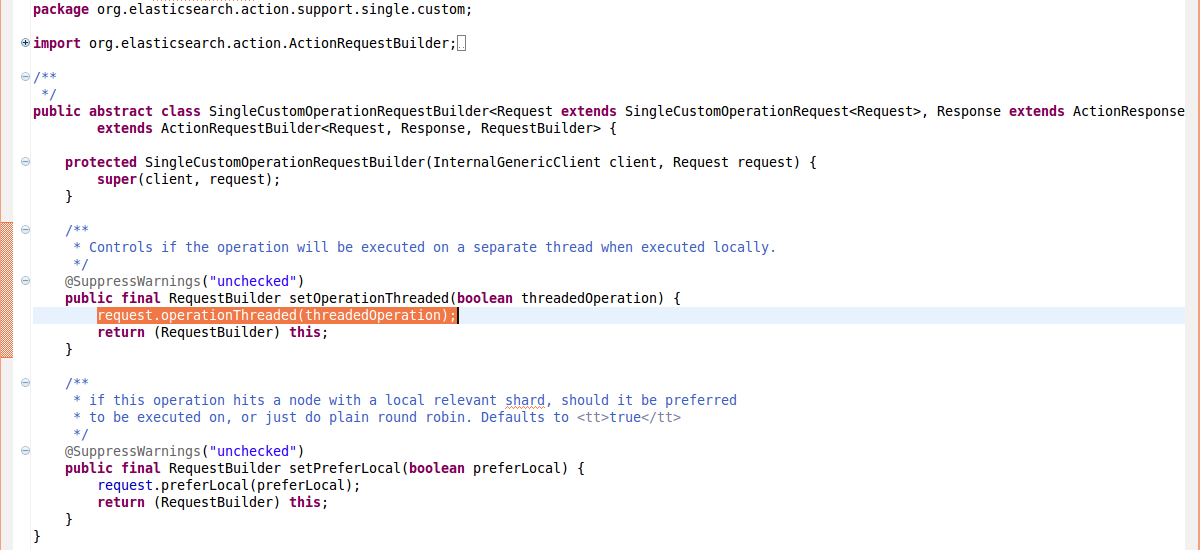
\includegraphics[width=\textwidth]{codingspectator-extract-method-selection.png}
%
\caption{\label{FigCodingSpectatorExtractMethodSelectionExample}A programmer
selects a piece of code to extract into a new method. The selected code is part
of class \texttt{SingleCustomOperationRequestBuilder} from commit
\texttt{bdb1992} of the open-source Elasticsearch project
(\texttt{https://github.com/elasticsearch/elasticsearch}).}
%
\end{figure}

\begin{figure}
%
\centering
%
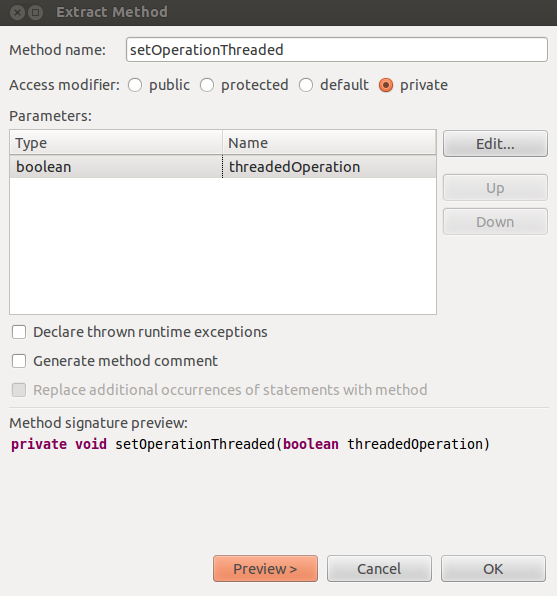
\includegraphics[width=0.5\textwidth]{codingspectator-extract-method-configuration.png}
%
\caption{\label{FigCodingSpectatorExtractMethodConfigurationExample}A programmer
configures an automated Extract Method refactoring by entering the desired name
of the new method.}
%
\end{figure}

\begin{figure}
%
\centering
%
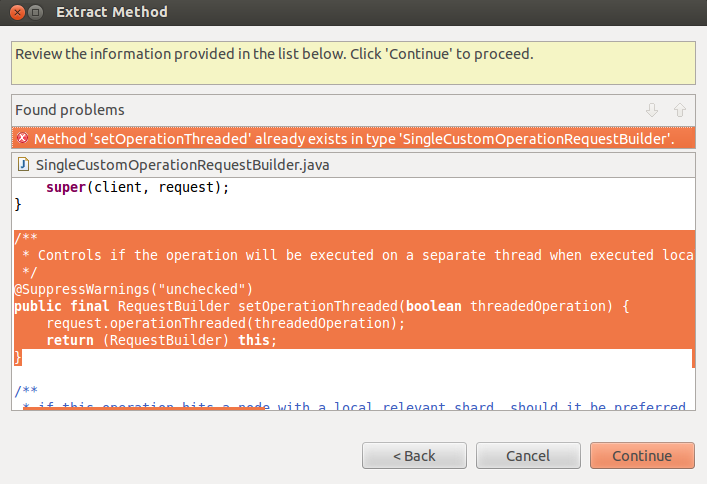
\includegraphics[width=0.6\textwidth]{codingspectator-extract-method-error.png}
%
\caption{\label{FigCodingSpectatorExtractMethodErrorExample}The Extract Method
refactoring reports a name conflict problem to the programmer. The programmer
can either ignore the problem and continue the refactoring, go back to the
configuration page to provide a different name, or cancel the refactoring.}
%
\end{figure}

\begin{figure}
%
\centering
%
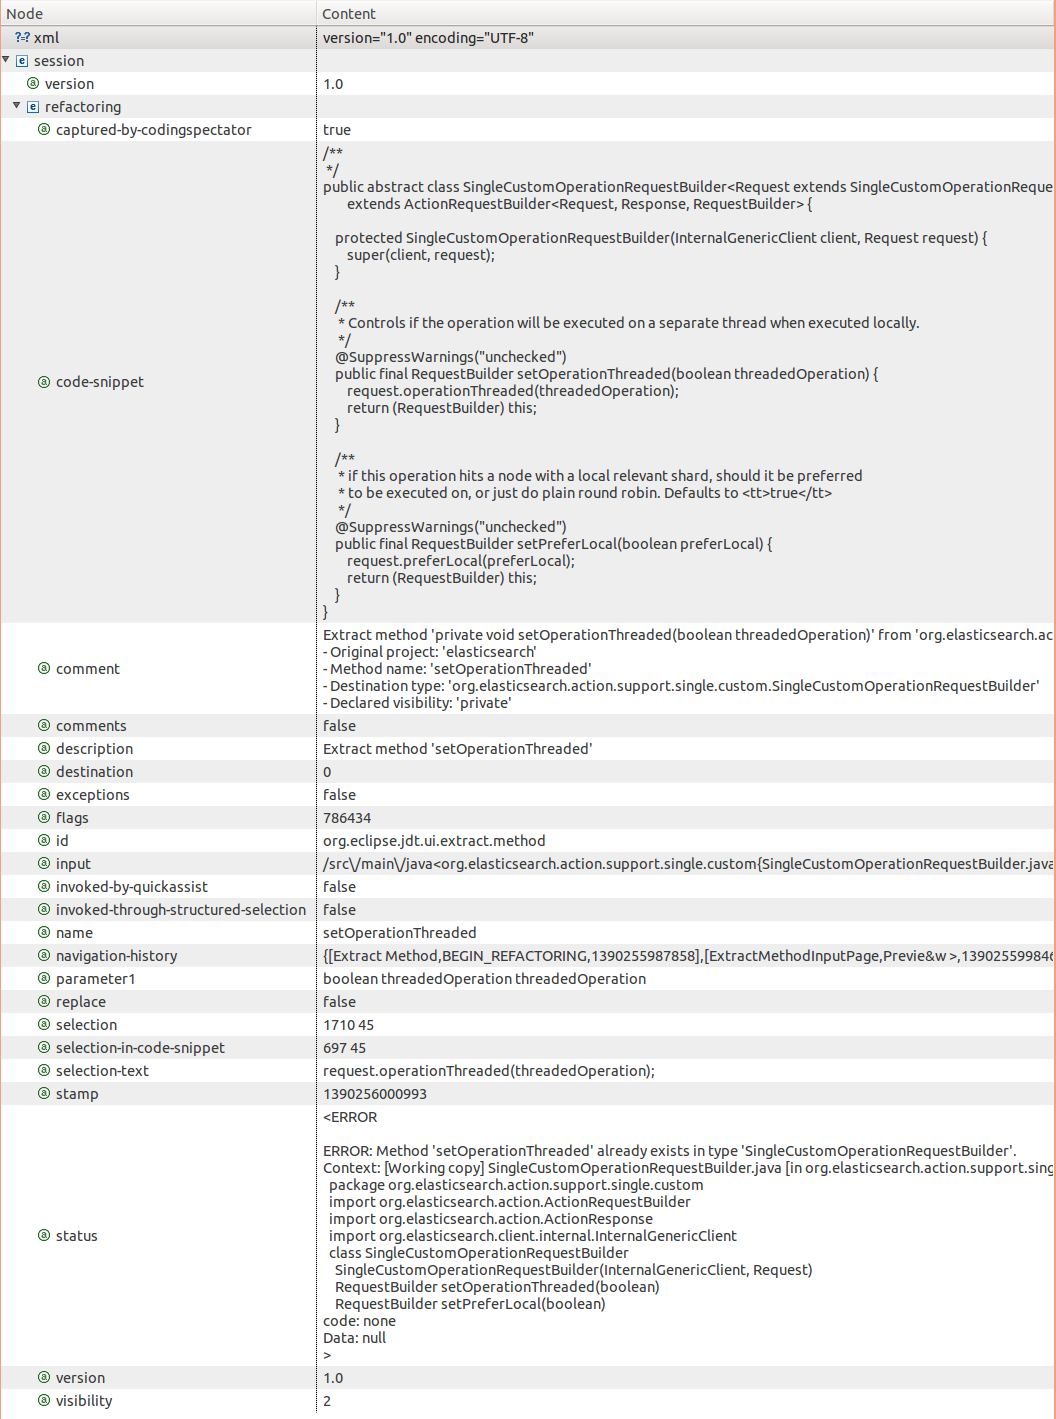
\includegraphics[width=\textwidth]{codingspectator-refactoring-xml.png}
%
\caption{\label{FigCodingSpectatorDescriptorExample}An example refactoring
descriptor recorded by \CodingSpectator.}
%
\end{figure}

\subsubsection{Deploying \CodingSpectator}

Deploying \CodingSpectator{} consists of two main steps:
%
\begin{inparaenum}[(1)]
%
\item setting up a Subversion repository and
%
\item setting up an Eclipse update site.
%
\end{inparaenum}

\paragraph{Setting Up a Subversion Repository}

\CodingSpectator{} regularly submits users' data to a central Subversion
repository. To collect \CodingSpectator's data automatically, you need to set up
a Subversion repository and create accounts for your users. To allow the users
to submit their data to the Subversion repository, you should grant them
appropriate write accesses to the repository.

Using a Version Control System such as Subversion as the data repository has
several advantages:

\begin{enumerate}
%
\item Subversion makes all revisions of each file easily accessible. This makes
  troubleshooting easier for researchers.
%
\item For textual files, Subversion submits only the \emph{changes} made to the
  files as opposed to the entire new file. This differential data submission
  leads to faster submissions.
%
\item There are libraries such as SVNKit\footnote{http://svnkit.com/} that
  provide an API for Subversion operations such as add, update, remove, and
  commit. \CodingSpectator{} uses SVNKit for submitting users' data to the
  central repository.
%
\item Setting up a Subversion server is a well-documented process. This avoids
  the burden of setting up a specialized server.
%
\end{enumerate}

On the other hand, a disadvantage of using Subversion as the data repository is
that it requires the users to maintain a copy of their data on their file
systems. The Subversion working copy on the users' systems takes \emph{space}
and can also cause \emph{merge conflicts}, \eg, if a user restores the contents
of the file system to an earlier version. To handle merge conflicts,
\CodingSpectator{} has built-in support for automatic conflict detection and
resolution. When \CodingSpectator{} detects a merge conflict, it removes the
user's data from the central repository and then submits the new data. Despite
removing the data from the central repository, the researchers can still locate
the merge conflicts and restore the data that was collected before the conflicts occurred.

\CodingSpectator{} prompts the users for their Subversion user names and
passwords when \CodingSpectator{} is about to submit their data.
\CodingSpectator{} gives the users the option to save their passwords in Eclipse
securely. See \url{http://codingspectator.cs.illinois.edu/documentation} for
more information about the features of \CodingSpectator{} for users.

\paragraph{Setting Up an Eclipse Update Site}

Users of \CodingSpectator{} install it from an Eclipse update
site\footnote{\url{http://codingspectator.cs.illinois.edu/installation}}. An
Eclipse update site is an online repository of the JAR and configuration files
that Eclipse requires for installing a plug-in.

You will have to customize \CodingSpectator{} at least by specifying the URL of
the Subversion repository to which \CodingSpectator{} should submit users' data.
You may also want to customize the message that \CodingSpectator{} shows to the
users when it prompts them for their Subversion credentials. You can customize
these aspects of \CodingSpectator{} by changing the configuration files that are
packed in the existing JAR files hosted at the Eclipse update site of
\CodingSpectator. If you need to customize \CodingSpectator{} in more complex
ways that involve changes to its source code, you should follow the instructions
for building \CodingSpectator's update site from source code.

\subsubsection{Extending \CodingSpectator}

In addition to collecting detailed refactoring data, \CodingSpectator{} provides
a reusable infrastructure for collecting Eclipse usage data. Extending
\CodingSpectator{} frees researchers from having to develop many features from
scratch, \eg, Subversion communications, automatic merge conflict detection and
resolution, secure storage of Subversion credentials, and periodic update
reminders.

\CodingSpectator{} provides an Eclipse extension point (id =
\texttt{edu.\-illinois.\-codingspectator.\-monitor.\-core.\-submitter}) and the
following interface:

\begin{lstlisting}
public interface SubmitterListener {
  // hook before svn add
  void preSubmit();
  // hook after svn add and before svn commit
  void preCommit();
  // hook after svn commit
  void postSubmit(boolean succeeded);
}
\end{lstlisting}

The above interface provides three hooks to \CodingSpectator's submission
process. \CodingSpectator{} checks out the Subversion repository into a folder,
which we refer to as the \emph{watched folder}. Then, it executes the Subversion
commands (\eg, add and commit) on the watched folder. A plug-in that extends the
\Code{submitter} extension point and implements the \Code{SubmitterListener}
interface can perform actions before or after two of the Subversion commands that
\CodingSpectator{} executes: add and commit.
%
For example, \CodingSpectator{} overrides the method \Code{preSubmit} to copy
the recorded refactoring descriptors to the watched folder. As another example,
the developers of \CodingSpectator{} made the Eclipse UDC plug-in use the
\Code{submitter} extension point and copy the UDC data to the watched folder. As
a result, \CodingSpectator{} submits the UDC data to the Subversion repository.
Effectively, this is an alternative method to the one presented in
\SecRef{SecUDCHowToUseIt} for collecting UDC data in a central repository.

%TODO: The paragraph above feels like a wrapup partiularly the last sentence.  Can you craft one more sentence with final words of advice to those who want to use Coding Spectator for their research?
% LocalWords: CodingSpectator Urbana Champaign IDE timestamp
%
% LocalWords: CodingTracker refactoring refactorings refactoring's
%
% LocalWords: SVNKit URL usernames online API



\subsection{Existing Data}

Existing UDC data is available through the Eclipse foundation at this URL:
\url{http://archive.eclipse.org/projects/usagedata/}
%could provide more analysis, maybe even BigData

\subsection{Exercises}

\begin{ExerciseList}
 \Exercise[type={long}, difficulty={0}]Define GQM? 
  \Answer Goal-Question-Metric is a methodology for refining a level goal into specific metrics to generate from data
 \Exercise[ type={long}, difficulty={1}]How is GQM Relevant to usage data collection? 
  \Answer It helps the researcher to identify a more specific set of IDE commands useful to their research so they do not have to track all commands in the IDE.
  \Exercise[ type={long}, difficulty={2}]Take an idea for usage monitoring and define a GQM for your idea. 
  \Answer Open-ended question asking students to apply the GQM method to their work.  Check to see that Goals are appropriate goal statements, questions refine the goal and lead the reader towards a specific measureable entity, and metrics are defined with all appropriate dimensions (such as time, and scale).
  \Exercise[ type={long}, difficulty={2}]Using your GQM, identify the usage data attributes you need to collect. 
  \Answer Open-ended question deriving a set of usage data elements from the student's defined GQM.  Usage data atrributes should consist of specific IDE commands, user actions within the editor, or another element measurable with soruce code and IDE access. 

\end{ExerciseList}


\subsection{Eclipse Mylyn Monitor}


\section{How to Analyze Usage Data}

Thus far we have been focusing on concrete usage data collection frameworks and the specific data collected by these frameworks. When analyzing this data, or data from other collection frameworks, data analysis follows several predictable patterns, which we discuss in this section. However, we first discuss the nature of the collected data, especially whether it is anonymous, which dramatically effects how it is analyzed.

\subsection{Types of Data}

\vspace{0.1in}

\noindent
{\bf Anonymous data}, where only records of activities and anonymous facts about artifacts are recorded, may at first seem strictly inferior. Indeed there are some limitations around what can be inferred from anonymous activity streams. Yet the advantages make it a great complementary data source. First, developers are receptive to data collection for research purposes, and thus the ability to collect a large amount of information from many developers increases greatly. Second, because of this larger collection, while it may be more difficult to analyze anonymous data, any conclusions made on a larger data set collected from working developers are ultimately more believable, as they represent actual field usage. 

In this section we focus on analyzing anonymous data sources. We do so because analyzing anonymous activity streams is similar to analyzing non-anonymous data streams (i.e., they are both activity streams) and because the unlimited variation of analysis permitted by non-anonymous data affords few generalities. As we discuss analyzing usage data we start with straightforward magnitutde analysis, build to a categorization system for activity streams, and finally discuss dividing streams into sessions. 


\subsection{Usage Data Format}
Most usage data is collected as an activity stream with varying levels of supporting detail. In Figure~\ref{fig:theoretical} we present an abstraction of a typical activity stream. It includes a timestamp, followed by the activity, appended with (often anonymous) details concerning that activity. We can apply this model to the examples discussed earlier. For instance, the Mylyn Monitor's interaction event corresponds to a row in our theoretical model. It includes a timestamp (i.e., StartDate), an activity description (i.e., Kind, OriginId), and additional information (i.e., StructureHandle, StructureKind). Similarly, the CodingSpectator example includes a timestamp (i.e., stamp), an activity description (i.e., id), and a much larger set of additional information (i.e., code-snippet, selection, selection-in-code-snippet, etc.). Because these and other usage data activity streams can easily be described using our abstraction we will refer to it as we describe data analysis techniques.


%TODO: Rewrite/Adapt/Remove this paragraph now that it's been integrated

%What do they look like

%include theoretical example

%several concrete examples (codingsepctator, Sando, Eclipse study)

%Software systems often keep a record about what event was completed (or not) in the form of a log file. The information collected in the log file is often used for diagnostic purposes. If a system failure occurs, the logs for that period can be inspected to see which sequence of events were executed by the system and what were the values for the dynamic information in those events. Each log line can be traced back to a particular line of code where the method to log this information was called. Hene, we can get complete information on what events were executed. The log message store information about the branches taken by that particular instance of execution and the values for variables in the code. Due to these reasons, the information in the log file is collected as a serially ordered flat text file. In short, a log file is a collection of log lines, with each of them having information about a single event, its time of execution and the dynamic information about variable values. Note that each log line may span across multiple lines, but provides information to distinct two adjacent log lines.



\begin{figure*}[t]
 \centering
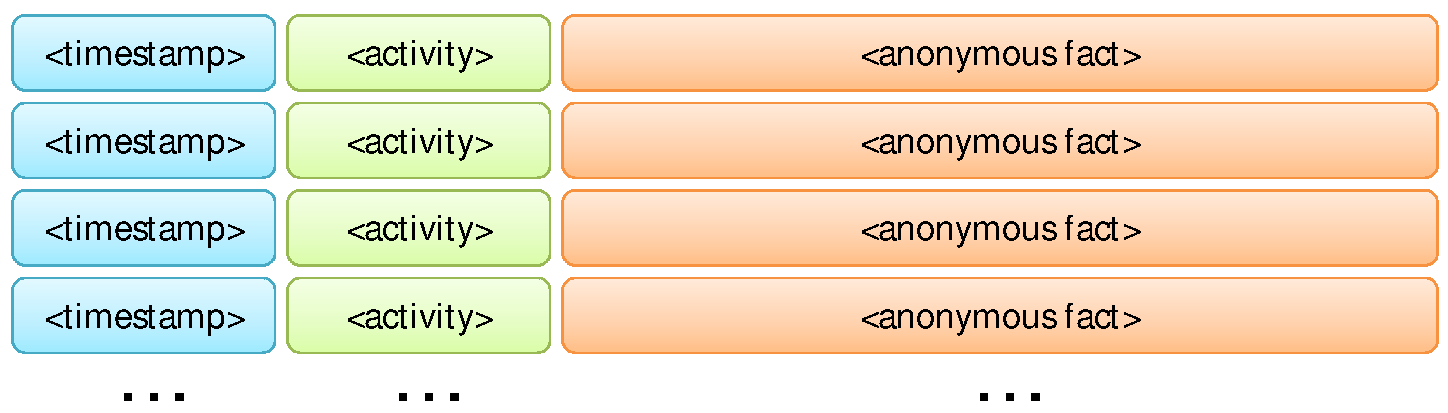
\includegraphics[width=1\columnwidth]{activityLogTheoretical.pdf}
\caption{Abstract model of developer activity streams.}
\label{fig:theoretical}
\end{figure*}



%\begin{figure*}[t]
 %\centering
%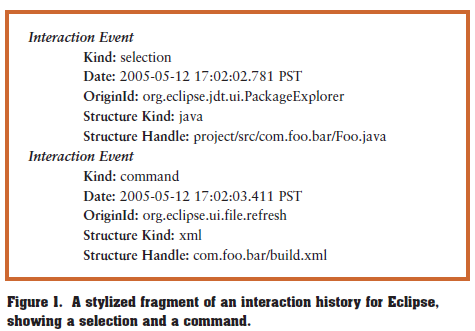
\includegraphics[width=0.5\columnwidth]{activityEvent}
%\caption{Activities as Captured in an Eclipse Usage Data Study}
%\label{fig:activity}
%\end{figure*}
%
%\begin{figure*}[t]
 %\centering
%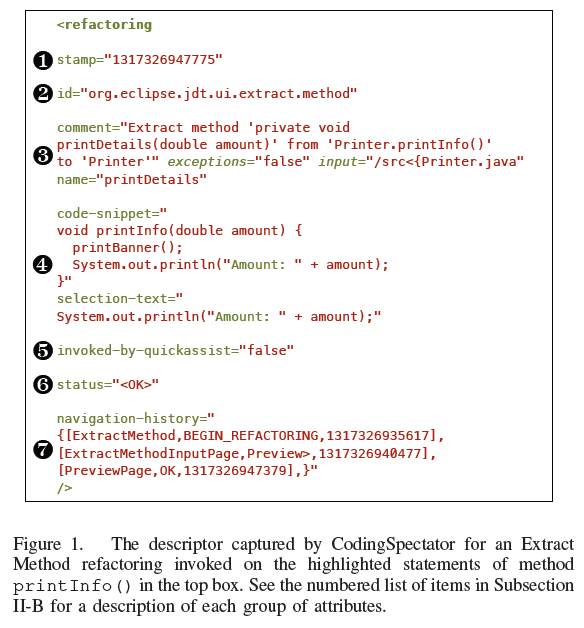
\includegraphics[width=0.5\columnwidth]{codingSpectator}
%\caption{Activities as Captured in a CodingSpectator Study of Refactoring Events}
%\label{fig:activit}
%\end{figure*}



\subsection{Magnitude Analysis}
A major advantage of anonymous usage data is the fact that it captures developers in their natural habitat, without any observational bias. Deriving conclusions from hours of developers' field work is naturally more convincing than from hour-long, in-lab user studies. One type of questions that usage data is well-suited to answer uses measurement of the magnitude of occurence of a specific event. For instance, researchers may want to know ``How often do developers invoke the pull-up refactoring'' or ``How often is the file search invoked?''. By performing a count of a specific message in the collected logs, researchers can easily calculate frequencies of specific actions that can be often sufficient to answer important research questions. However, researchers must be wary of a few common issues with magnitude analysis. First, in any sufficiently large set of user logs there is a small set of users that will use the feature/tool under analysis orders of magnitude more often than the general population, potentially skewing the data. Second, any fine-grained attempt to qualify the raw counts requires making possibly incorrect assumptions about the data. For instance, there is a temptation to report refactorings per hour, yet any fine-grained time calculation requires assumptions about how time was spent between activities, which experience has taught us are often wrong. Note that coarse-grained qualification, such as refactorings performed per day, are possible.   

%example
\begin{figure}
  \centering
  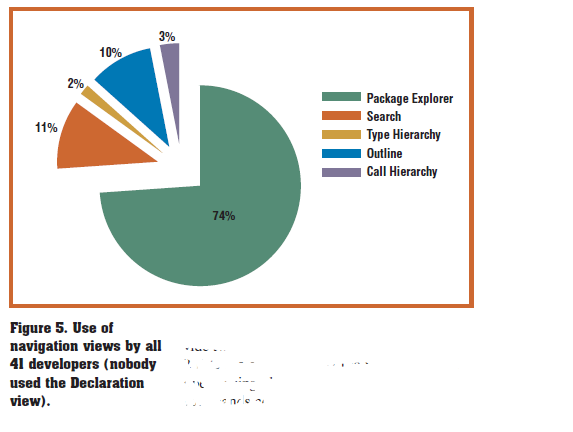
\includegraphics{AnalyzingUsageData/eclipse}
  \caption{Breakdown of Navigation-Focused View Usage in Eclipse}\label{fig:eclipse}
\end{figure}




\subsection{Categorization Analysis}
While magnitude analysis is well-suited for answering research questions about the use of a single IDE command, many research questions are related to a specific part or tool in the IDE, which usually corresponds to multiple IDE commands. For instance, the research question ``How often are refactorings performed?'' cannot be answered via magnitude analysis alone, as refactorings can be triggered through a number of different IDE commands. These commands first need to be categorized, after which magnitude analysis can be used. When focusing on a concrete sub-task, such as refactoring, it may be easy to categorize activities. In this case, all refactoring commands, such as pull-up or extract method, can be classified as refactorings. However, when focusing on more general behavior, such as editing, navigating, and searching, categorization can be difficult. It is impossible to say, for instance, from a single click in the {\tt File Explorer} window, whether that click represents a search, as the developers browses a few promising files, or a navigation, as he implicitly opens a type declaration of a variable he was just browsing. Thus, categorization without context can produce noisy data in certain cases. However, caterigorization is a powerful tool, especially when there is little ambiguity in the IDE commands that are analyzed.

To illustrate both the power and limitations of category analysis consider the following IDE data stream, and the research questions ``Do developers use code search tools?''. 

\begin{verbatim}
Collector Started
2014-02-02 13:21:22 - User submitted query to Find-in-Files
2014-02-02 13:24:36 - Find-in-Files retreived 42 results
2014-02-02 13:32:21 - User clicked on result 2
2014-02-02 13:46:56 - User submitted query to Quick Find
2014-02-02 14:07:12 - Open definition command; input=class
...
2014-02-02 14:46:52 - User submitted query to Find-in-Files
2014-02-02 14:46:56 - Find-in-Files retreived 8 results
2014-02-02 14:48:02 - Click on File Explorer
...
\end{verbatim}

For this research question, the category of log events related to code search tools should be identified and counted. Modern IDEs commonly offer several code search tools, which operate at the global or local scale, such as the {\tt Find-in-Files} and
the {\tt Quick Find} tools in the above example based on Visual Studio. Using categorization analysis we can identify three
log events related to usage of code search tools, and report various statistics aimed at answering the research question (e.g. number of code search events per day, number of code search events per user). However, the IDE usage data can sometimes be affected by noise, which cannot be avoided by categorization analysis. For instance, the second query to {\tt Find-in-Files} is not followed by a user click, which is a failed interaction with the {\tt Find-in-Files} tool and should likely not be included in answering the research question.


%\begin{figure*}[t]
%\centering
%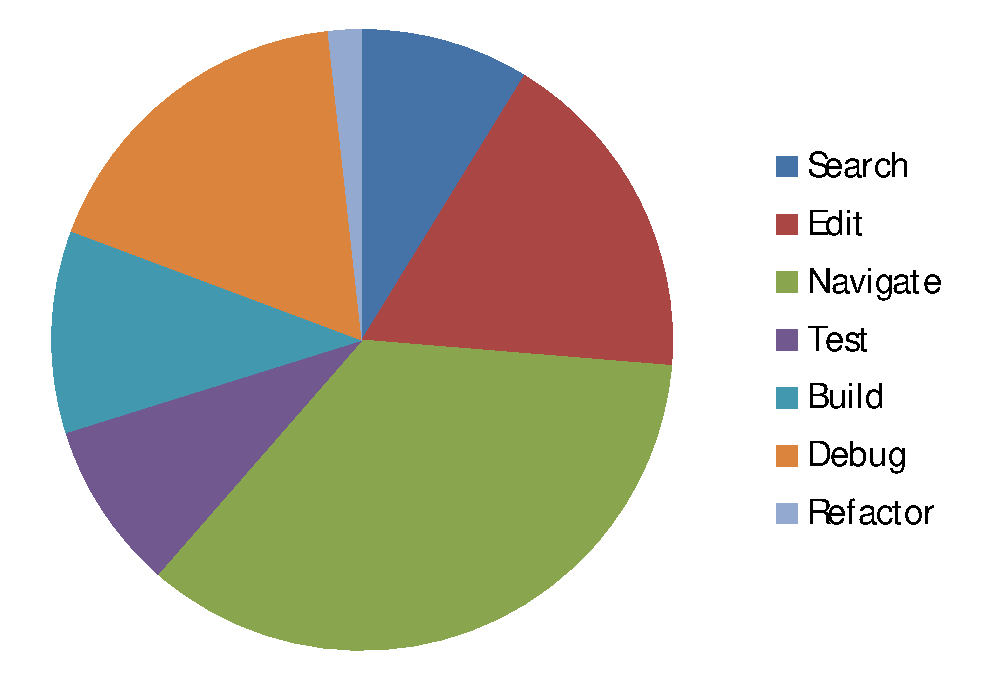
\includegraphics[width=0.5\columnwidth]{../Graphics/activityCategorization.pdf}
%\caption{Pairwise matches across categories, including matching and mismatching pairs.}
%\label{fig:category}
%\end{figure*}


\subsection{Sequence Analysis}
%intro to seqence analysis, sessions
Magnitude analysis and categorization are both appropriate for answering simple research questions. However, a more powerful way of analyzing activity logs is through sequence analysis, which first breaks activity sequences into session, according to some criteria, and then reports upon characteristics of that session. A session is a particular interaction with an IDE by a specific user in order to complete a task (e.g. refactoring, looking for a starting point for a maintenance task, etc.), consisting of all of IDE events in a given time span.
For instance, answering the research question of ``Are developers successful at finding initial points in the code for a software maintenance task?'' requires that the sequence of IDE events corresponding to each maintenance task be identified, before we can perform further analysis using either magnitude or categorization analysis. The granularity of a session is determined by the guiding research question. For certain research questions, we may be interested in a smaller session (e.g. searching the code base), while for others we may need to consider a longer time span (e.g. performing a maintenance task, developing a new feature). 

%how difficult or easy is it to determine sessions
In many cases, extracting sessions from activity sequences can be challenging as it impossible to know exactly when a developer begins or ends a particular task, without understanding his or her underlying thought process. There are several possibilities in how session extraction can be performed, based on the task related to the specific research question. One possibility is to use sentinels, which are specific actions where we can detect a task begins or ends. For instance, in code search, submitting a query to the code searcht tool begin one task and end the prior task in the activity stream. Another possibility is to use the passage of time to extract sessions, where time without any activity is used as a signal of task start or finish. Coman et al.'s \cite{Coman-TaskIdent} algorithm uses a combination of key events in the activity stream and time distance between such events to extract relevant sessions corresponding to developer tasks. In lab validation studies this algorithm has shown very high accuracy (80\%) when compared to the ground truth reported by developers, however this accuracy may not hold up in an industrial setting\cite{Zou-ComanIndustry}.


%example
As an example of sequnce analysis, consider a researcher investigating finding initial points in the code for a software maintenance task. Specifically, the developer is interested in the following research question ``Are users satisfied with file search results?''. This question, while impossible to answer via simple magnitude analysis can be investigated via session analysis. Using assumptions from in-lab studies that show that opening a search result followed by a long pause correlates with user satisfaction we can analyze activitiy logs to determine how often user behavior indicated satisfaction in the field. The researcher may break activity logs into sessions, starting with a search being executed and ending on the last interaction with that result set. He could calculate additional characteristics from this raw data, such as the amount of time spent per session, the number of results reviewed, and the number of files opened.   


\begin{figure*}[t]
 \centering
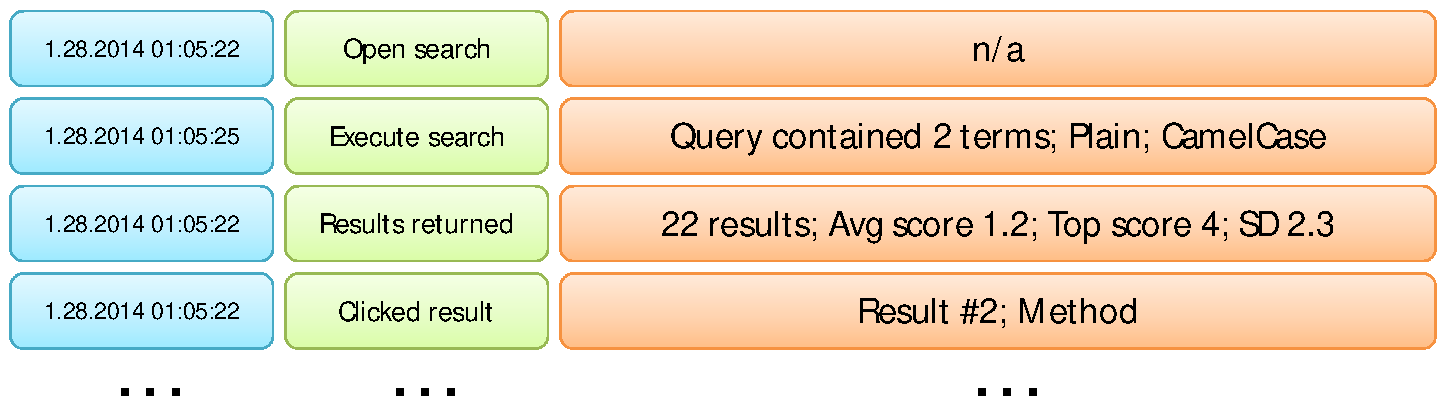
\includegraphics[width=1\columnwidth]{../Graphics/activityLogActual.pdf}
%\caption{Pairwise matches across categories, including matching and mismatching pairs.}
\label{fig:actual}
\end{figure*}

%Sequence analysis is currently the most powerful tool we have for analyzing logs. While there has been preliminary work to complete annotate activity logs into tasks or even states (e.g., editing, searching, navigating, testing, etc.) these analyses are currently unreliable. In fact, we believe that because user behavior is often multi-purposed there will remain major obstacles to inferring higher-level user states from activity streams, ultimately limiting the usefulness of any full log analysis. 




\subsection{State Model Analysis}
Another way to analyze log data is to view the log as a sequence of events occurring in a state machine.  Using state models, we can quantify the occurrences of repeating actions and describe a usage pattern in statistical analysis.  In state model analysis, the sequential data is converted to nodes and edges of a graph which represents the entire data in states and transitions between them.  A Markov state model provides information about the probability of occurrence of each state and the transitional probability of each activity.   The statistics provided in a Markov state model include the quantity of time and probability for the developer being in each state.  From a given state, the model calculates the probability of each transition to different unique states.  State models answer specific questions such as what is the probability that once a developer searches the code, they edit a code element listed in the find results. Expanding this question, the probability of an entire use case or set of transitions through the usage model, is calculable from the state model.  

State model graphs make it easy to identify the most active states and edges provides information about the important activities in the data set.  As the number of states increases, the WDG becomes more complex and hence difficult to understand.  When this occurs, summarizing the detailed event data into higher-level categories effectively combines the states to get more meaningful information.   For example, classifying events in usage data of similar types into categories results in fewer states with the same number of transitions as the original data.

We generate a state model from a usage log by transforming the serially ordered events in a sequence data to a Weighted Directed Graph (WDG) data structure.  We can abstract the information in the log line to any level, such as, event level, event category level, tool level, or application level. In the sequence data, each event is important as a standalone event, however, in the WDG representation, the importance shifts to adjacent pairs of events. 
%We do this type of a transformation to record the order in which events happened. 
Therefore, each unique event in the sequence data is represented by a unique node in the WDG. 

To understand how to interpret a state model, look at our example graph figure \ref{op-profile-example}.  We see that an edge exists from one node (head) to another (tail) if there is an occurrence of the event representing the tail node immediately after the event representing the head node in the  log file. For example if event B follows event A in the log file, then there is directed edge from node A to node B in the WDG. The edges are labeled with the number of times this transition has occurred.  For example if B occurs a fifty times after A in the log file, then the edge from node A to node B in the WDG is labeled with 50. Typically, we keep track of the actual count as the weight of the edge, when building the graph. In the graph we display the percentage value as the label. This percentage is proportional to the total number of transitions.  The cumulative probability of out-edges of a node is 1. The transitional probabilities of each out-edge is calculated by dividing the number of transactions of that out-edge with the sum of all outward transactions from that node. We could also store the dynamic parameter information in each log line as a list along the edges. 

As an example, consider a sample log file shown in figure \ref{samplelogfile} given below and the corresponding state model graph in figure \ref{op-profile-example}. Intuitively you can see how the state model represents the log states and transitions between them in the sequence of events.  

\begin{figure}
\hrulefill
\begin{verbatim}
2013-03-21 18:18:32Z,A
2013-03-21 18:18:33Z,B
2013-03-21 18:20:49Z,C
2013-03-21 18:20:50Z,A
2013-03-21 18:20:56Z,B
2013-03-21 18:20:57Z,A
2013-03-21 18:21:08Z,C
2013-03-21 18:21:08Z,D
2013-03-21 18:21:08Z,E
2013-03-21 18:21:08Z,A
\end{verbatim}
\hrulefill
\caption{Sample Log File to Convert to State Model}\label{samplelogfile}
\end{figure}

\begin{figure}[h]
  \centering
  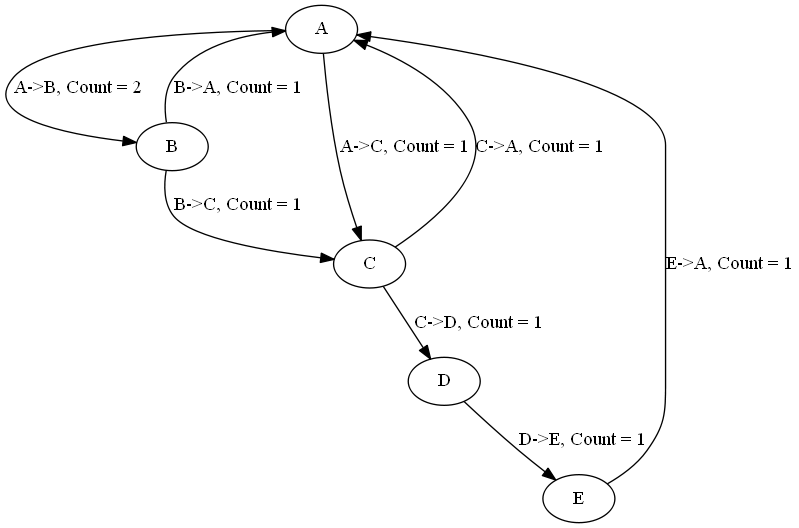
\includegraphics[scale=.40]{op-profile-example.png}
  \caption{Weighted Directed Graph of the Example Log}\label{op-profile-example}
\end{figure}






%the other example is aligned with the sample graph thus better.
%As an example of WDG, consider a simple log file where the activities are separated by commas. $1-2, 2-3, 3-4, 4-5, 5-4, 4-5, 5-4, 4-6, 6-7, 7-5, 5-4, 4-5, 5-4, 4-5, 5-8, 8-9$. The events in the log file are mapped to their corresponding event IDs: $1, 2, 3, 4, 5, 4, 5, 4, 6, 7, 5, 4, 5, 4, 5, 8, 9$. Each node is a unique event. An edge between nodes 1 and 2 signifies that the event 2  appears after event 1  in the log file. The labels on the edges have the actual count and could have the transitional probabilities as well. The transitional probability from node 1 to node 2 is 1.0, whereas the transitional probability from node 4 to node 6 is 0.2.  This is depicted in Fig \ref{op-profile-example}.
 
Converting a log into a state model requires three steps.  We use JUMBL (Java Usage Model Builder) from the Software Quality Reasearch Laboratory (SQRL) of the University of Tennessee.    Details on input formats and JUMBL tools are available on sourceforge at \footnote{\url{http://jumbl.sourceforge.net/}}.
\begin{enumerate}
\item
First, convert the log file into a representation for each transition called a sequence based specification. The format for a sequence based specficicaiton in csv files is described in the JUMBL user guide. This representation contains the following information with one row for each transition :
\begin{itemize}
\item State transition
\item Count of transitions
\item Total time elapsed
\item State In information
\item State Out information
\end{itemize}

\item
After importing the sequence based spec, JUMBL can write out the representation of a state model as a TML script or several other formats including GML (Graph Modeling Language) that graph tools can import.  The TML  has information about the nodes, the out edges from each node along with the number of transitions from each node to another. The corresponding graph for the usage log example is depicted in Fig. \ref{op-profile-example}
\end{enumerate}


Using state models, a sequence data with hundreds of thousands of lines can be quickly converted to more meaningful graphical representation using this method. Once the TML file is generated, we can use JUMBL to find out the state probabilities of each states. Using the state probability and the usage patterns we can draw conclusions about the occupancy of individual states and the use cases that involve transitions through several states.

%Trying this on without the following examples.  They don't really add much and raise more questions than they answer.  I hope reference take care of the how to in this case.


%
%\begin{figure}
%\label{sampleTML}
%\hrulefill
%\begin{verbatim}
%($ fill(1) $)
%model testlog
%//use this before each transition to show probability ($0.10$)
%
%source [A]
%($2$)"Count=2 (A->B), TimeElapsed= 7secs" [B]
%($1$)"Count=1 (A->C), TimeElapsed= 11secs" [C]
%
%[B]
%($1$)"Count=1 (B->C), TimeElapsed= 136secs" [C]
%($1$)"Count=1 (B->A), TimeElapsed= 1secs" [A]
%
%[C]
%($1$)"Count=1 (C->A), TimeElapsed= 1secs" [A]
%($1$)"Count=1 (C->D)" [D]
%
%[D]
%($1$)"Count=1 (D->E)" [E]
%
%[E]
%($1$)"Count=1 (E->A)" [A]
%
%
%"exit" [Exit]
%
%end 
%\end{verbatim}
%\hrulefill
%\caption{Sample TML for a State Model}
%\end{figure}



%%I commented these out because they were out in space in the document and not well supported by the text.  You probably cut the text because of other comments.  Anyhow does it make sense to stick with one WDG example based on the state model shown in text above?  Seems OK to me so far. 

%\begin{figure}
%  \centering
%  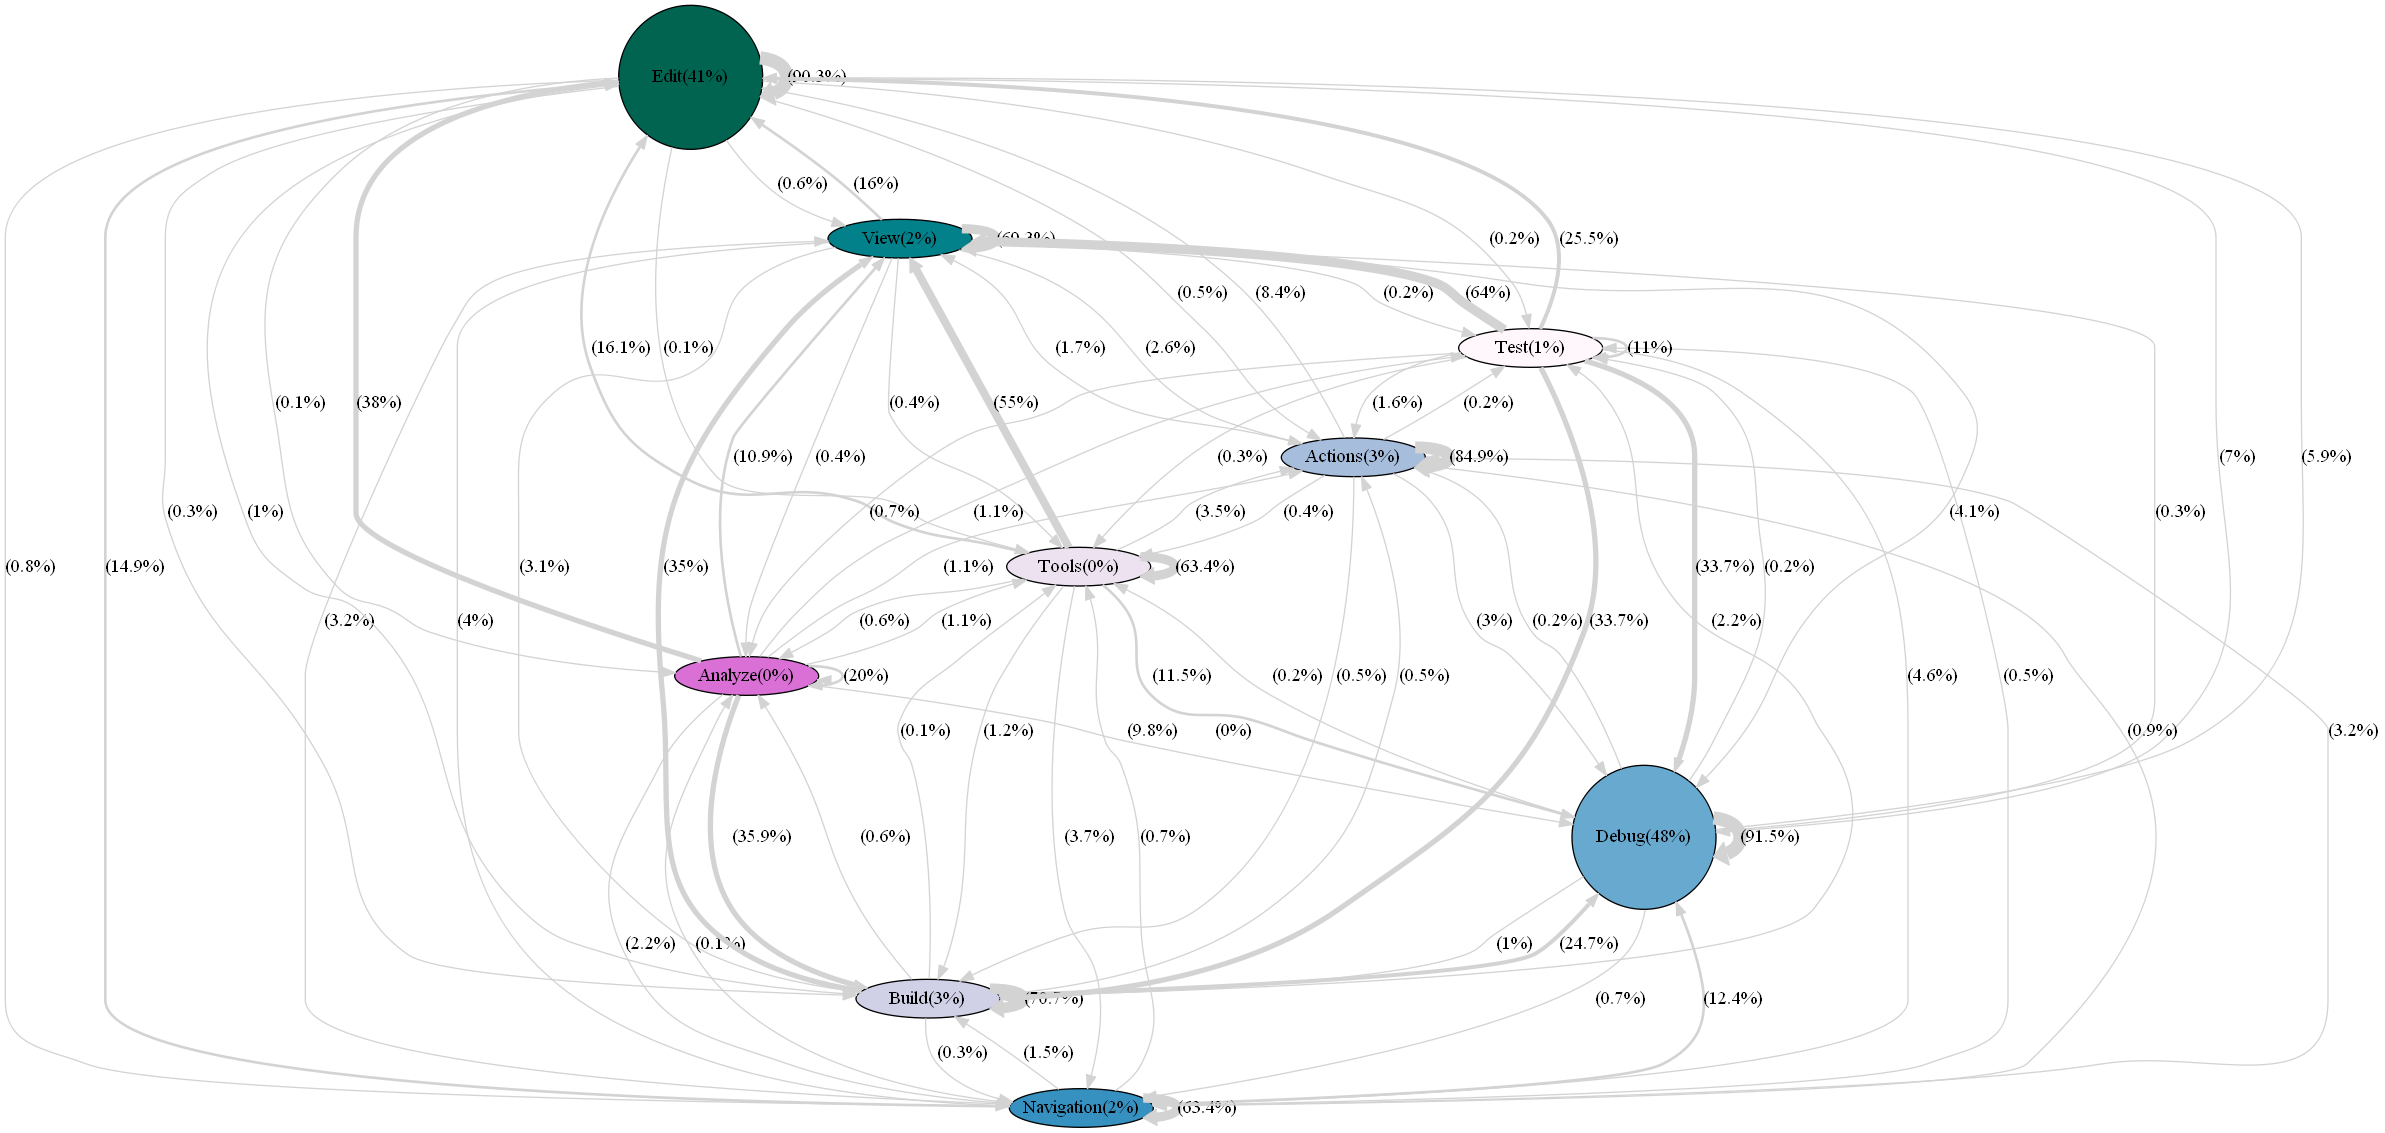
\includegraphics[scale=.15]{log_with_color.png}
%  \caption{WDG example with probability}\label{fig:log_with_color}
%\end{figure}

%\begin{figure}
%  \centering
%  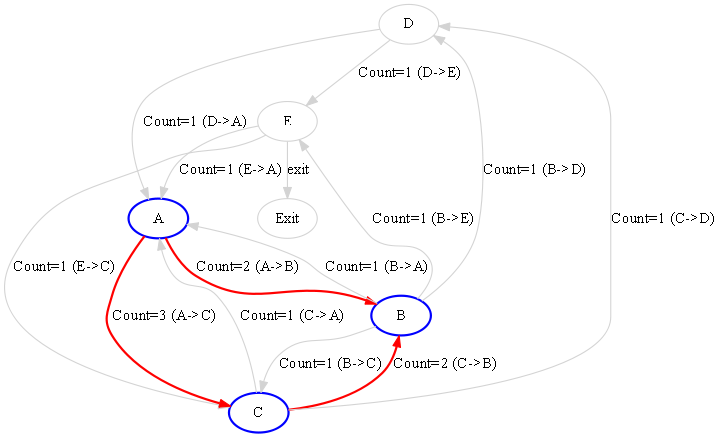
\includegraphics[scale=.50]{sample_log.png}
%  \caption{WDG example with count}\label{fig:sample_log}
%\end{figure}

 




\subsection{Research combining usage data with other sources}

\section{ Reasearch combining usage data with other sources}

  \begin{enumerate}
  \item Tasks 
  \item Change history
  \item Program elements
  \item News feeds
  \end{enumerate}
\section{ Perspectives on Data Analysis}


\begin{enumerate}
\item Creating and communicating developer oriented feedback
\begin{itemize}
	\item
	Identifying developer viewpoints of the data
	\item
	Designing a data visualization for developers
	\item
	Issues of privacy or sensitivity of data for developers
\end{itemize}
\item Tailoring usage data to provide value to toolsmiths
\begin{itemize}
	\item 
	Tool usage data
	\item 
	Analyzing contextual data relevant to tool use such as prior actions or follow-on actions, 
	\item 
	Determining whether tool use was successful.
\end{itemize}
\item Research perspectives and opportunities
\begin{itemize}
	\item
	Ideas to study IDE usage include debugging tasks, task oriented, navigation, reading
\end{itemize}

\end{enumerate}
\section{ Reasearch combining usage data with other sources}

  \begin{enumerate}
  \item Tasks 
  \item Change history
  \item Program elements
  \item News feeds
  \end{enumerate}
\section{Limits of What You Can Learn from Usage Data}\label{sec:limitations}

  \begin{enumerate}
  \item - 
  \item -
  \end{enumerate}
\section{A Look Ahead}

If the last two decades could be labeled the era
of big data collection, 
the next two decades will surely be labeled as the 
era of smarter big data analysis.
Many questions still remain:
How do we balance data privacy and data richness?
What are the long term effects of developer monitoring?
How can we maximize the value of data collection
for as many researchers as possible, and reduce the 
strain on research participants?
Answering these questions will help our research
community advance in usage data collection and analysis.

Usage data, while now widely collected, still remains largely 
an untapped resource by practitioners and rearchers.
In this chapter, we have explained how to collect and 
anlayze usage data, which we hope will help you ``stand
on the shoulders of giants'' and increase the ease
with which you can collect and analyze your own usage data.

\pagebreak
%\section*{Table of Contents}
%\begin{enumerate}
%  \item What Is Usage Data and Why Analyze It?
%  \item How to Collect Data or Get Pre-Existing Data
%  \begin{enumerate}
%  \item Data sources
%  \item Building Data Collection %(Dave and Kosta)
%  \item Instrumenting the IDE %(Will \& ?)
%  \item Video studies %(?)
%  \item Other methods
%  \end{enumerate}
%  \item How to Extract Attributes from Usage Data
%  \begin{enumerate}
%  \item Creating meaningful classification of events
%  \item Defining useful and balanced sequences % (Will, Anil)
%  \item Dealing with multi-event dependent sequences
%  \item  Modeling sequences with state models %(Anil)
%  \end{enumerate}
%\item{Perspectives on Data Analysis}
%\begin{enumerate}
%\item Creating and communicating developer oriented feedback
%\item Tailoring usage data to provide value to toolsmiths
%\item Research perspectives and opportunities
%\end{enumerate}
%\item Reasearch combining usage data with other sources 
%  \begin{enumerate}
%  \item Tasks 
%  \item Change history
%  \item Program elements
%  \item News feeds
%  \end{enumerate}
%  \item Limits of What You Can Learn from Usage Data 
%  \item A Look Ahead
%\end{enumerate}

  
\bibliographystyle{abbrv}
\bibliography{paper_id1} 

\end{document}

